\documentclass[10pt,xcolor={usenames},fleqn,serif]{beamer}
\listfiles

%% colors
\definecolor{darklava}{rgb}{0.28, 0.24, 0.2}
\definecolor{bittersweet}{rgb}{1.0, 0.44, 0.37}
\definecolor{brilliantlavender}{rgb}{0.96, 0.73, 1.0}
\definecolor{antiquefuchsia}{rgb}{0.57, 0.36, 0.51}
\definecolor{violetw}{rgb}{0.93, 0.51, 0.93}
\definecolor{Veronica}{rgb}{0.63, 0.36, 0.94}
\definecolor{atomictangerine}{rgb}{1.0, 0.6, 0.4}
\definecolor{darkgray}{rgb}{0.66, 0.66, 0.66}
\definecolor{brightcerulean}{rgb}{0.11, 0.67, 0.84}
\definecolor{cadmiumorange}{rgb}{0.93, 0.53, 0.18}
\definecolor{ochre}{rgb}{0.8, 0.47, 0.13}
\definecolor{midnightblue}{rgb}{0.1, 0.1, 0.44}
\definecolor{lemon}{rgb}{1.0, 0.97, 0.0}
\definecolor{grey}{rgb}{0.7, 0.75, 0.71}
\definecolor{amber}{rgb}{1.0, 0.75, 0.0}
\definecolor{almond}{rgb}{0.94, 0.87, 0.8}
\definecolor{bf}{RGB}{88, 86, 88}
\definecolor{bb}{RGB}{177, 177, 177}
\definecolor{blue(pigment)}{rgb}{0.2, 0.2, 0.6}
\definecolor{darkpastelgreen}{rgb}{0.01, 0.75, 0.24}

%%%%%%%%%%%%%%%%%%%%%%%%%%%%%%%%%%% importa pacchetti
\usepackage{usepkg}
\usepackage{mybiblatex}
%%%%%%%%%%%%%%%%%%%%%%%%%%%%%%%%%% Beamer set up
\usepackage{beamersetup}
%%%%%%%%%%%%%%%%%%%%%%%%%%%%%%%%%%% Funzioni generali
\usepackage{functions}
%http://tex.stackexchange.com/questions/246/when-should-i-use-input-vs-include
\newcommand{\setmuskip}[2]{#1=#2\relax} %%problem usinig mu with calc (req by mathtools) loaded
\usepackage{sources}
%\usepackage{length}
%%%%%%%%%%%%%%%%%%%%%%%%%%%%%%%%%%% Funzioni per questo file main
\usepackage{mathOp}
\def\status{coazione}%ripeter
\def\keeptrying{coazione}
\usepackage{LocalF}
%%%%%%%%%%%%%%%%%%%%%%%%%%%%%%%%%
\title{Popolazioni planetarie sintetiche}
% A subtitle is optional and this may be deleted
\subtitle{Osservazioni degli esopianeti. Scenario core accretion. Modelli di formazione planetaria globale.}
%\author{F.~Author\inst{1} \and S.~Another\inst{2}}
%\institute[Universities of Somewhere and Elsewhere] % (optional, but mostly needed)
\date{\today}
\subject{Seminario popolazioni planetarie settembre}
% This is only inserted into the PDF information catalog. Can be left
% out. 
% Delete this, if you do not want the table of contents to pop up at
% the beginning of each subsection:
%\input{tikzdir}%%contain tikz files as filecontents
\begin{document}

\begin{frame}
  \titlepage
\end{frame}
% Section and subsections will appear in the presentation overview
% and table of contents.
%\frame{\tableofcontents[onlyparts]}

\begin{frame}{TOC}
\tableofcontents[onlyparts]
\end{frame}

\part{Scenario e scopo}
\begin{frame}{caratteriatiche sistemi planetari e condizioni iniziali}
caos e probabilit\'a
\end{frame}

\begin{wordonframe}{Mordasini18 MAIN RESULTS}
\begin{itemize}
\item Cosa ho messo nel modello e2e? (Montecarlo variables) Disk metallicity $[M/H]$ (Santos 05) and $f_{dg}$ (Lodders 03). Initial disk mass: stability (SHu 90), observation (andrws 10, manara 16) MMSN; Disk lifetime (Haisch 01, mamajek 09); starting embryos position
planetesimal size is 300m, planetesimal distro $\propto r\expy{-1.5}$ and outer exponential radius half that of gas to account inward drift (kornet 01; birnstiel andrews 14) and more concentrated distro resulting from planetesimal formation (drazkowska 16) - ''The TW Hya Disk at \SI{870}{\micro\meter}:  Comparison of CO and Dust Radial Structures'' 2011; planetesimal size 300m: what's influenced?
Struttura disco accrescimento: calibrazione tempo di vita, evoluzione viscosa ed evaporazione - $\alpha=0.002$.
Evoluzione embrioni: accrescimento, evoluzione orbitale (N-body+migration timescale+e,i damping)

\item Distribuzione massa pianeti: distribuzione bimodale con discrimine a $30\mearth{}$.
\begin{figure}[!ht]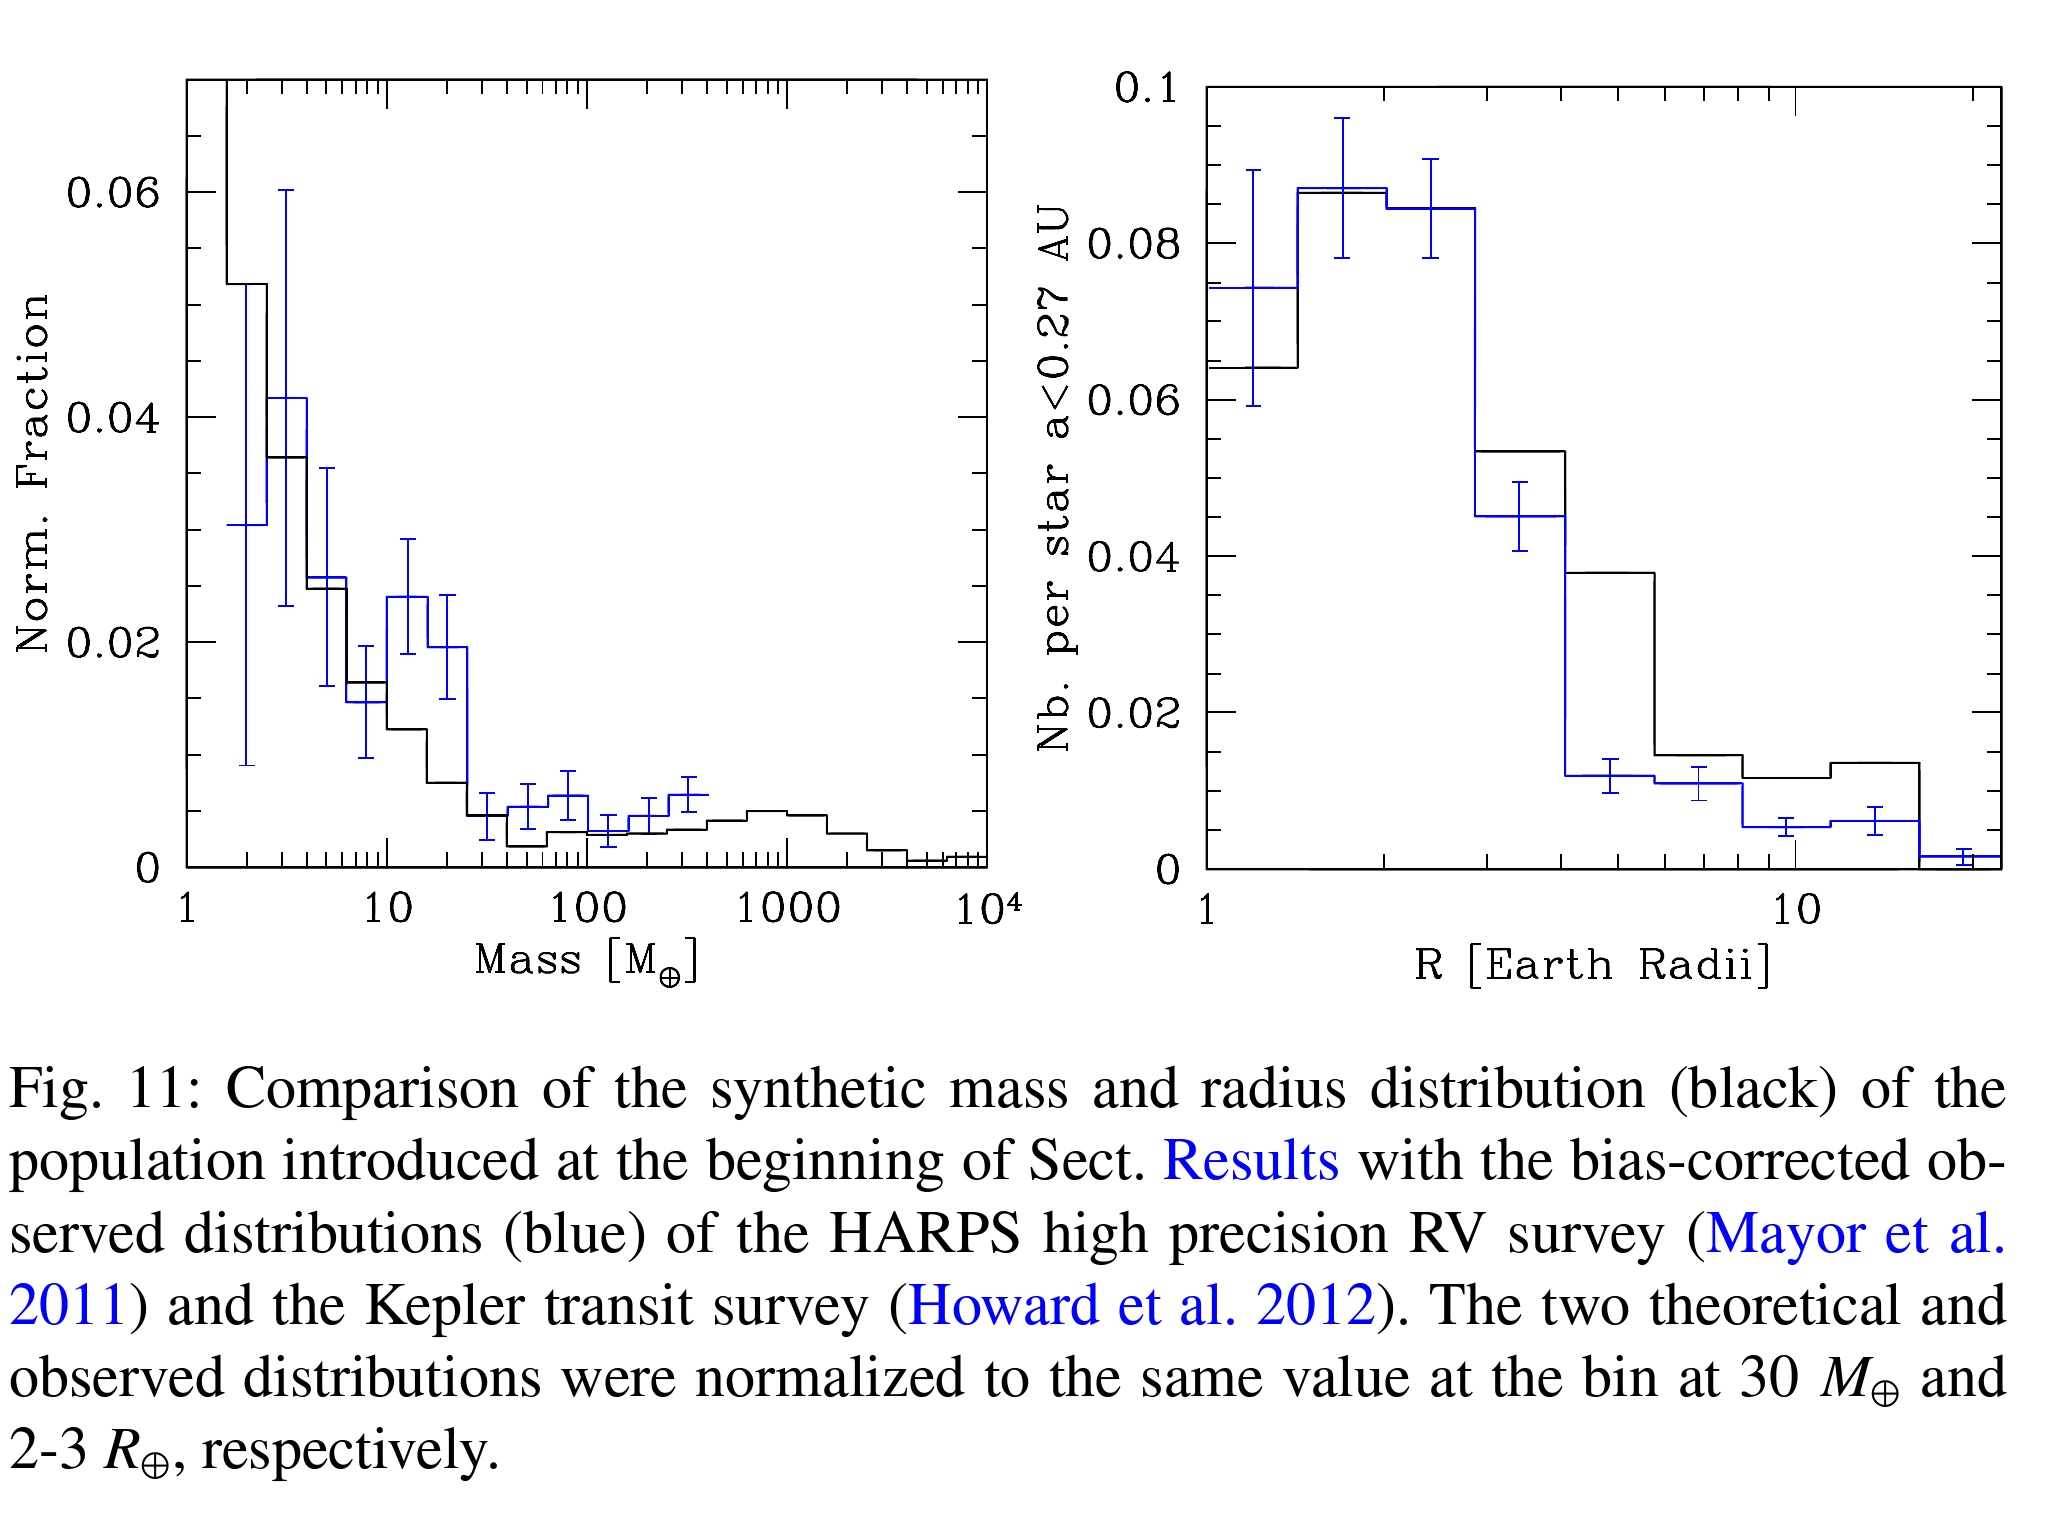
\includegraphics[trim={0cm 17cm 0 0},clip, keepaspectratio,width=0.9\textwidth]{MR-freq-obssynth}\caption{Distribuzioni di massa e raggio per popolazione planetaria sintetica (linea nera) e distribuzioni osservate tramite RV e transiti (linea blu) corrette per i bias. Da \cite{mordasini2018planetary}.}\label{fig:MR-freq-obssynth}\end{figure}
Massa critica per accrescimento di gas: tempo scala accrescimento planetesimi vs tempo scala disco.
Tempi scala migrazione
\item distribuzione in semiassi che dipende da posizione iniziale embrione: necessity to include earlier planetary formation; montecarlo variable: initial starting position embryos- kokubo ida 00: uniform distro in log(a) (vedi anche ida lin 10) (dov'era scritto del comportamento caotico??+); hasegawa pudritz 11, cridland 16: embryos rapidly moves into traps.
Preferred formation regions of planetesimal (Drazkowska16; brauer 08), particle pile-up outside orbits of already existing planets (Pinilla15), strong migration traps (Horn 12, Hasegawa Pudritz 12).
Disc/planetesimals parameters: planetesimal has steeper profile $\propto r\expy{-3/2}$, outer exponential radius half that of gas: inward drift of dust (kornet 01, birnstiel Andrews 14), concentrated distro resulting from planetesimal formation (Drazkowska 16);
\item Distribuzione raggi: diagramma massa-raggio, composizione, evaporazione.
\item (Mordasini pg 27) LArge majority are low mass planets ($0.1-10\mearth{}$), 
\item frequency of giant, close-in and habitable planets. The high frequency of close-in planets can be reproduced assuming steep distribution of planetesimal and centrally concentrated (chiang laughlin 13, drazkowska 16)
\item correlation with disk properties (mordasini 12a): metallicity effects (mortier13)
\item Sub-saturn mass desert (ida lin 04) not seen in kepler data (Thompson 18): accretion of planetesimal slow down gas accretion
\item migrazione, cattura risonante: ''On the migration of two planets in a disc and the formation of mean motion resonances'' Migaszewski 15; ''Perturbation of compact planetary systems by distant giant planets'' Hansen 17
\end{itemize}
\end{wordonframe}

\begin{frame}[label={intro}]{Popolazione esopianeti osservati e scopo popolazioni sintetiche}
\begin{figure}[!ht]
	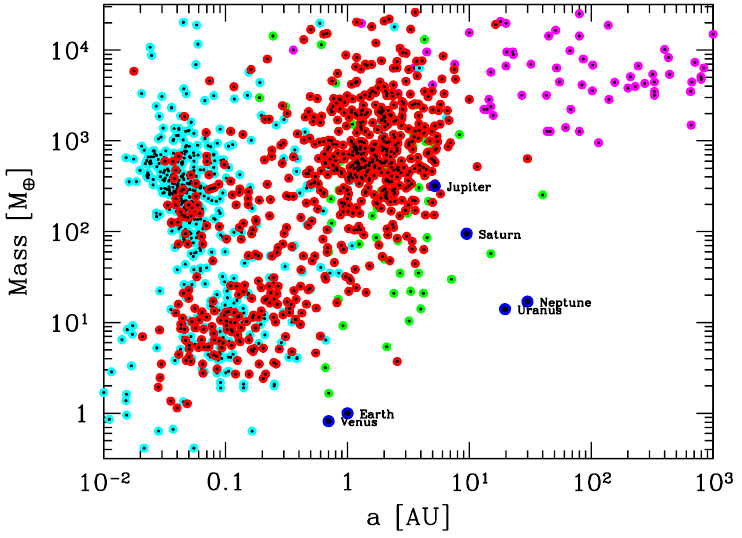
\includegraphics[trim={0cm 0 0 0},clip, width=0.75\textwidth]{obsMa}
	\caption{Diagramma massa-distanza degli esopianeti in ''The extrasolar planet encyclopedia''. Rosso, celeste, magenta e verde sono pianeti rivelati tramite RV, T, osservazione diretta e microlensing. Da \cite{mordasini2018planetary}.}\label{fig:Maplot}
\end{figure}
\end{frame}

\begin{wordonframe}{Popolazioni planetarie sintetiche: doppio ruolo sistema solare, survey RV (mass metallicity period distro), T(radius) ...}
In questo seminario ho studiato come si costruisce una popolazione sintetica. L'obiettivo (della simulazione di popolazione planetaria) \'e generare una popolazione planetaria che sia in accordo con le osservazioni a partire da combinazione casuale di condizioni iniziali del disco protoplanetario.(Si parametrizzano le condizioni iniziali il cui valore \'e distribuito in accordo alle osservazioni)

In questa slide \'e rappresentata la popolazione osservata nel diagramma massa-distanza: la posizione di un pianeta nel diagramma riflette la sua storia di formazione, migrazione (ed evoluzione dinamica). Gli esopianeti sono distribuiti su ampia regione del diagramma con regioni pi\'u dense o dove c'\'e minore popolazione: spesso una moltitudine di fenomeni concorre alla forma della distribuzione di esopianeti che \'e possibile individuare con simulazione end to end del processo di formazione.
(Su cosa mi sono concentrato?)

Ho considerato lo scenario di formazione planetaria di core accretion cercando le caratteristiche tipiche nella distribuzione delle propriet\'a della popolazione..

Core accretion (bottom-top) coagulazione polvere ed eventualmente accrescimento gas, mentre lo scenario alternativo parte dagli addensamenti causati dall'instabilit\'a G del disco.

[Il sistema solare per primo \'e stato il banco di prova delle teorie di formazione di sistemi planetari: loscenario di core accretion trova giustificazione in alcune caratteristiche del sistema solare]

\end{wordonframe}

\begin{wordonframe}{Coazione vs obiettivo - tempo come?}
ritmo concetto parola
\end{wordonframe}

\begin{wordonframe}{Concretezza}
Definire paths!! - argomenti - mio obiettivo: materiale a disposizione, veloce ripasso beamer fatti
Sistema solare: modello nebulare: punti a favore di core accretion. Massa e tempi scala formazione: struttura orbitale  e tempi accrescimento gas urano nettuno (Mass distribution and planet formation in the solar nebula).
Popolazione esopianeti: survey RV, T. RV: osservabili, Harps survey, bias osservativi e completezza, distribuzioni massa, distanza orbitale e metallicit\'a stellare. T: osservabili e bias osservativi, kepler, distribuzione periodo e raggio, relazione massa-raggio: densit\'a media.
\end{wordonframe}

\part{Vincoli osservativi. Sistema solare e popolazione esopianeti. (Quali dati osservativi deve riprodurre un modello di formazione palnetaria: da sistema solare a distribuzione statistica propriet\'a esopianeti)}\linkdest{RV-Texo}
\begin{frame}{Sistema Solare e scenario core accretion}
\begin{columns}[T]
	\begin{column}{0.45\textwidth}
	\begin{itemize}
			\item Arricchimento metalli
			\item Oggetti pi\'u antichi hanno et\'a del Sole %($\Omega\tau_{cool}\gg1$): 
			\item numerosa popolazione corpi minori
		\end{itemize}
	\end{column}
	\begin{column}{0.54\textwidth}
		\begin{table}[!ht]
			\begin{flushleft}
\begin{minipage}{.25\linewidth}
	\begin{tabular}{@{}|ccc|@{}}
		\hline
		&\parbox{1.5cm}{Jupiter $317.8\mearth{}$}&\parbox{1.5cm}{Saturn $95.1\mearth{}$}\\
		$M_c$&$0-11\mearth{}$&$9-22\mearth{}$\\
		\hline
		$M_Z$&$1-39\mearth{}$&$1-8\mearth{}$\\
		\hline
		$M_Z^{tot}$&$8-39\mearth{}$&$13-28\mearth{}$\\
		\hline
		$Z/Z_{\odot}$&$1-6$&$6-14$\\
		\hline
	\end{tabular}
\end{minipage}%

\vspace{3mm}
			
			\begin{minipage}{.25\linewidth}
				\centering
				\begin{tabular}{@{}|ccc|@{}}
					\hline
					&\parbox{1.5cm}{Uranus $14.5\mearth{}$}&\parbox{1.5cm}{Neptune $17.1\mearth{}$}\\
					\hline
					$M_{rock}$&$3.7\mearth{}$&$4.2\mearth{}$\\
					\hline
					$M_{ice}$&$9.3\mearth{}$&$10.7\mearth{}$\\
					\hline
					$M_{H/He}$&$1.5\mearth{}$&$2.2\mearth{}$\\
					\hline
				\end{tabular}
			\end{minipage}
					\end{flushleft}
			\caption{Da \cite{baraffe2009physical}.}\label{tab:JSUNcomp}
		\end{table}
	\end{column}
\end{columns}
\end{frame}

\begin{wordonframe}{''ruoli sistema solare'' e intro CA}
[Il sistema solare per primo \'e stato il banco di prova delle teorie di formazione di sistemi planetari: loscenario di core accretion trova giustificazione in alcune caratteristiche del sistema solare e da quest'ultimo \'e possibile stimare in maniera quantitativa la massa del disco protoplanetario da cui ha avuto origine]

I meteoriti pi\'u antichi hanno et\'a compatibile con et\'a del sole quindi \'e plausibile che si siano formati per primi e nello scenario CA trovano collocazione naturale il resto dei corpi minori.
La composizione di giove, saturno e dei pianeti ghiacciati mostra un sostanzioso arricchimento di metalli rispetto al sole: questo sarebbe ovvia conseguenza dell'accrescimento di gas su core solido.

\end{wordonframe}

\begin{frame}{Minimum mass solar nebula}
\begin{columns}[T]
	\begin{column}{0.45\textwidth}
\begin{itemize}
	\item Massa prevista nei modelli GI due ordini di grandezza superiore a MMSN ($Q\gg1$)
\end{itemize}
	\end{column}
	\begin{column}{0.54\textwidth}
			\begin{figure}[!ht]
			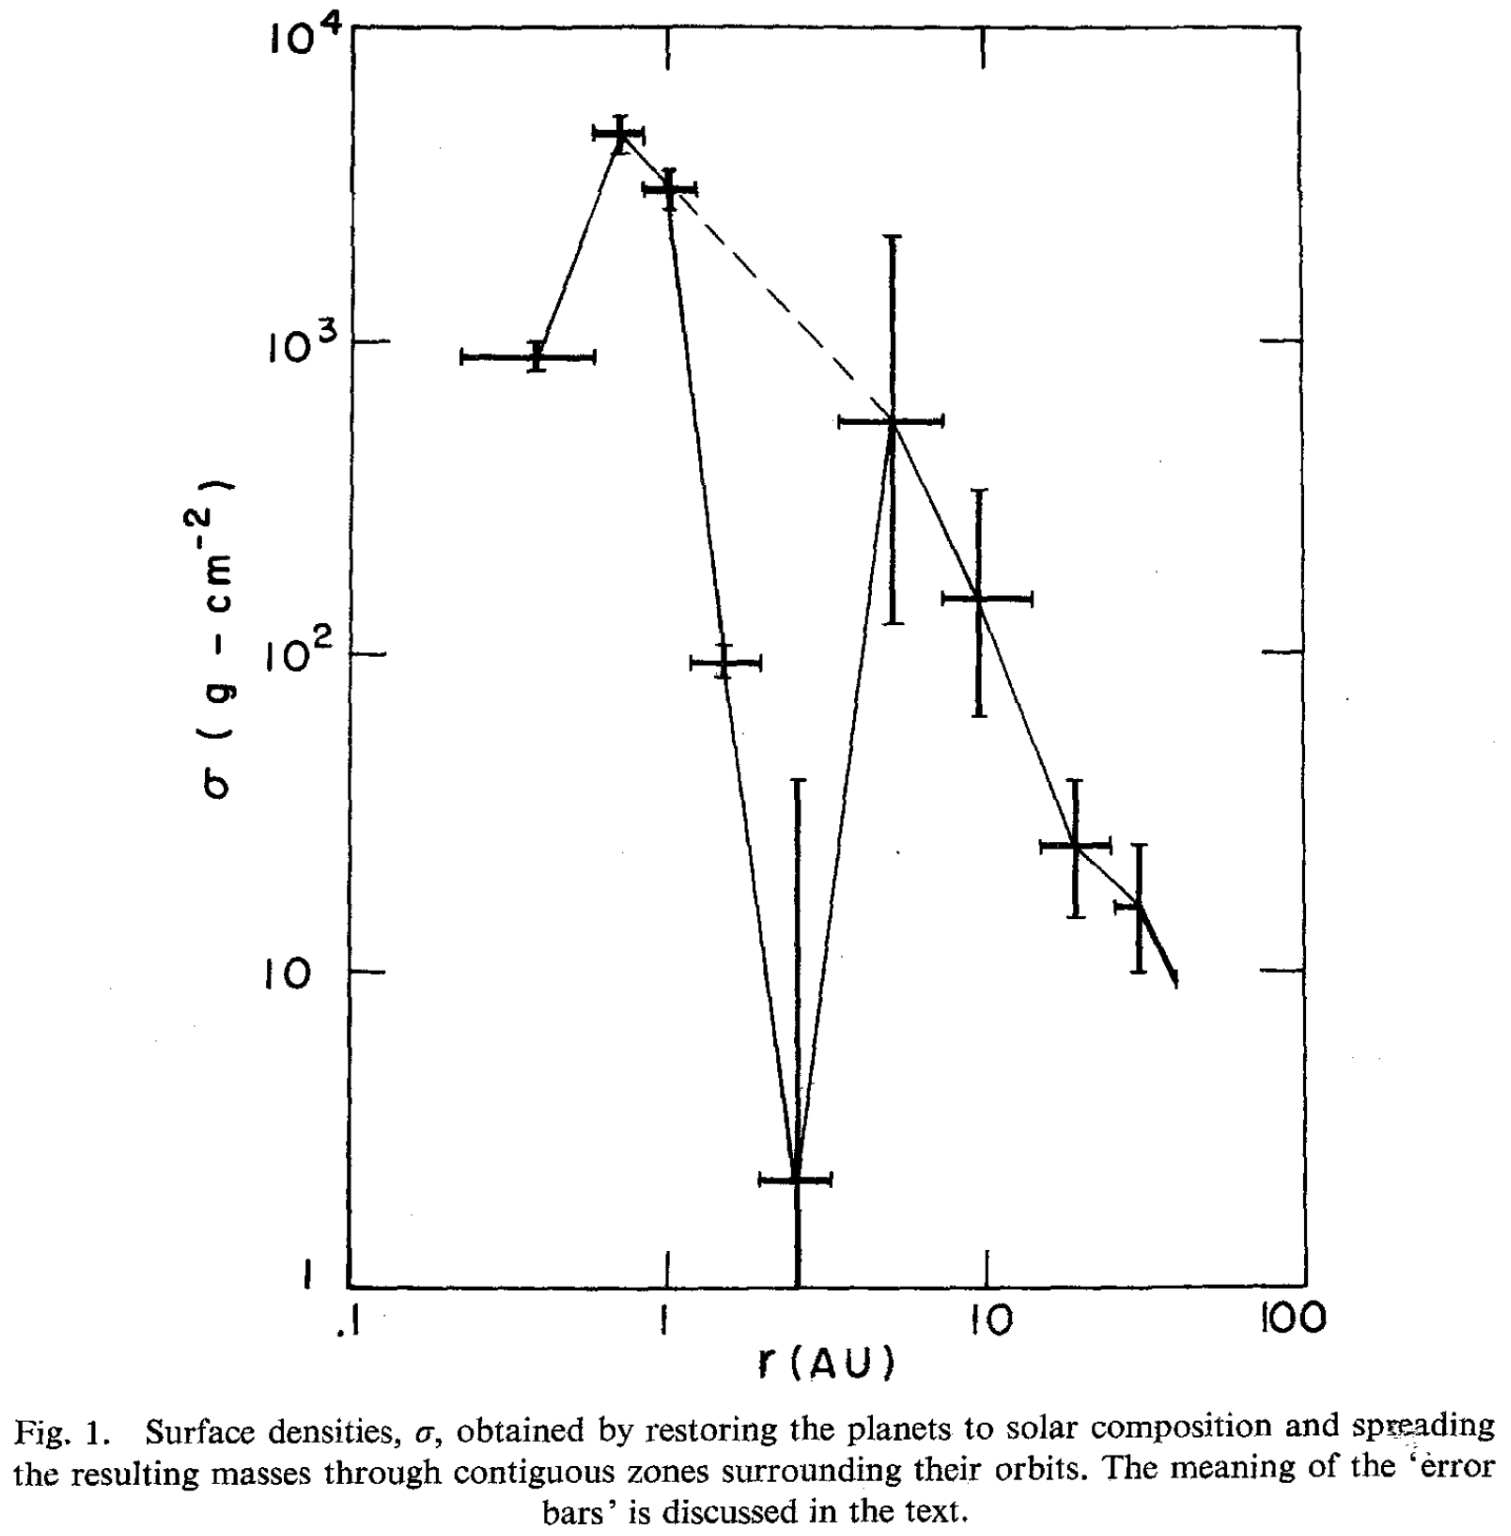
\includegraphics[trim={0cm 5cm 0 0cm},clip, width=0.99\textwidth]{Snebuladensity}
			\caption{Da \cite{weidenschilling1977distribution}.}\label{fig:Snebuladensity}
		\end{figure}
	\end{column}
\end{columns}
\end{frame}

\begin{wordonframe}{Core accretion e MMSN}

Inoltre \'e possibile determinare dalla configurazione attuale,aggiungendo la massa di H/He per ripristinare composizione solare, una stima inferiore della massa iniziale 
\begin{align*}
&\Sigma\propto r\expy{-3/2}
&M\approx0.02\msun{}
\end{align*}

\end{wordonframe}

\begin{frame}{Survey: HARPS}
\begin{figure}[!ht]
	\centering
	\begin{subfigure}[b]{0.37\textwidth}
		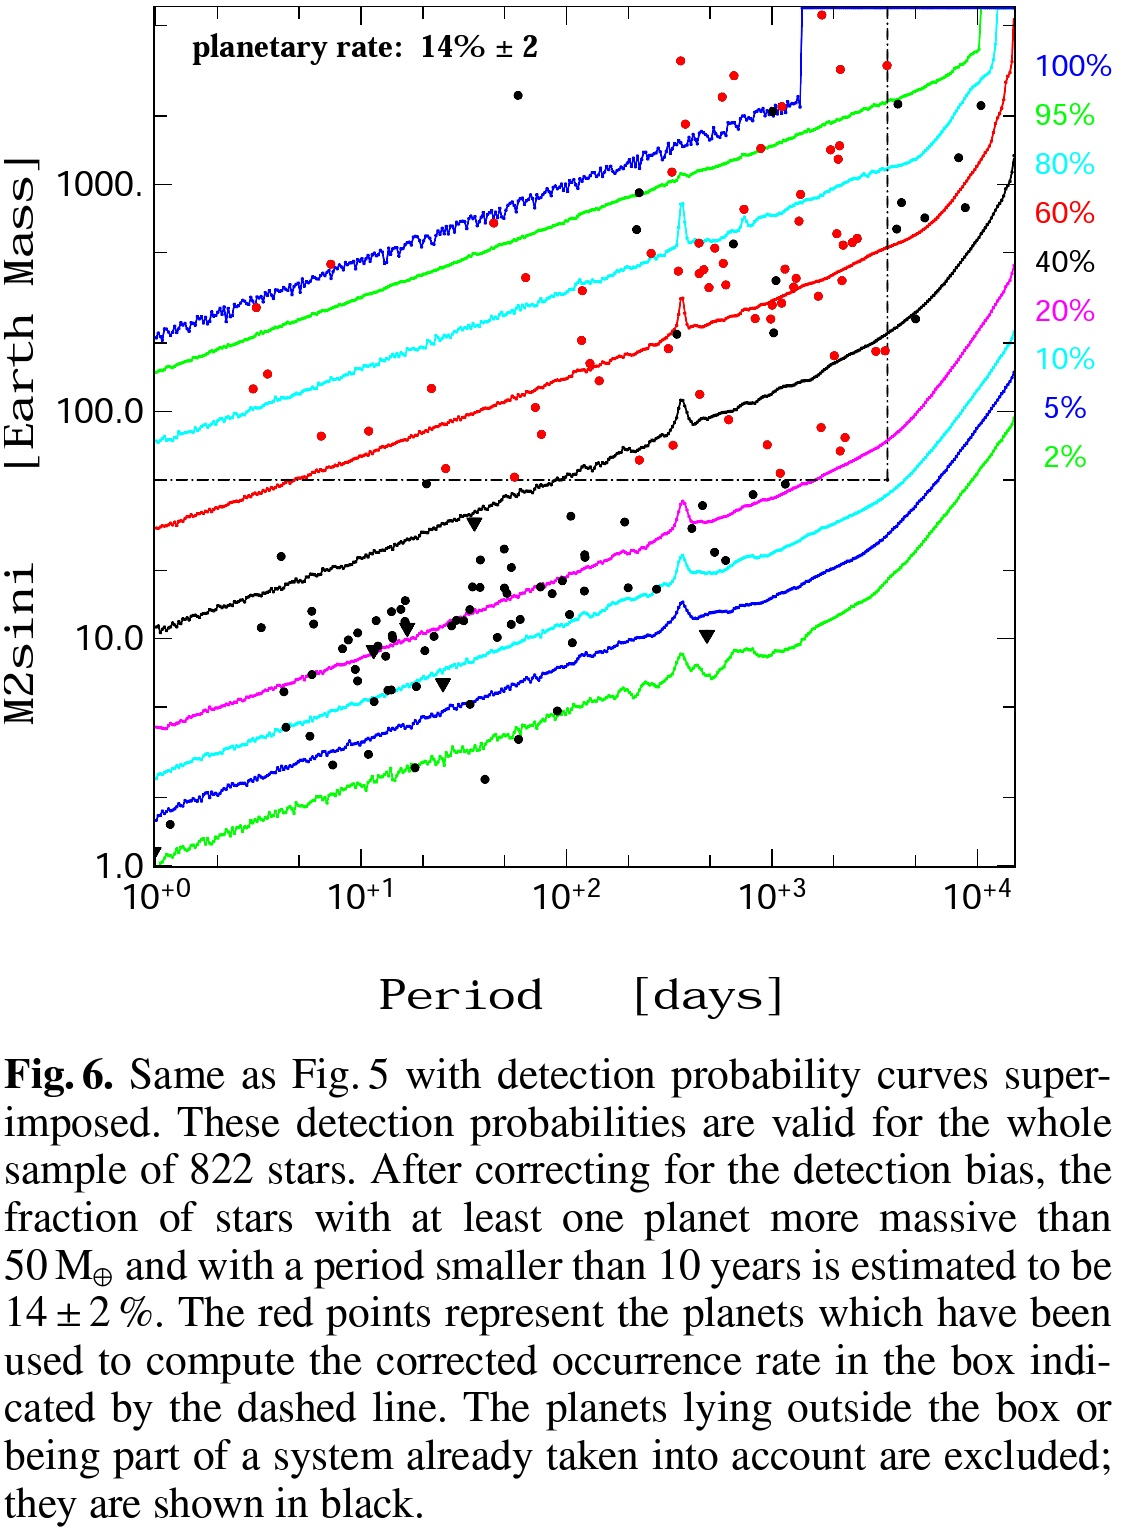
\includegraphics[trim={0cm 17cm 1cm 0},clip, width=0.99\textwidth]{PMfreq-e23}\label{fig:PMfreq-e23}
	\end{subfigure}
	~
	\begin{subfigure}[b]{0.37\textwidth}
		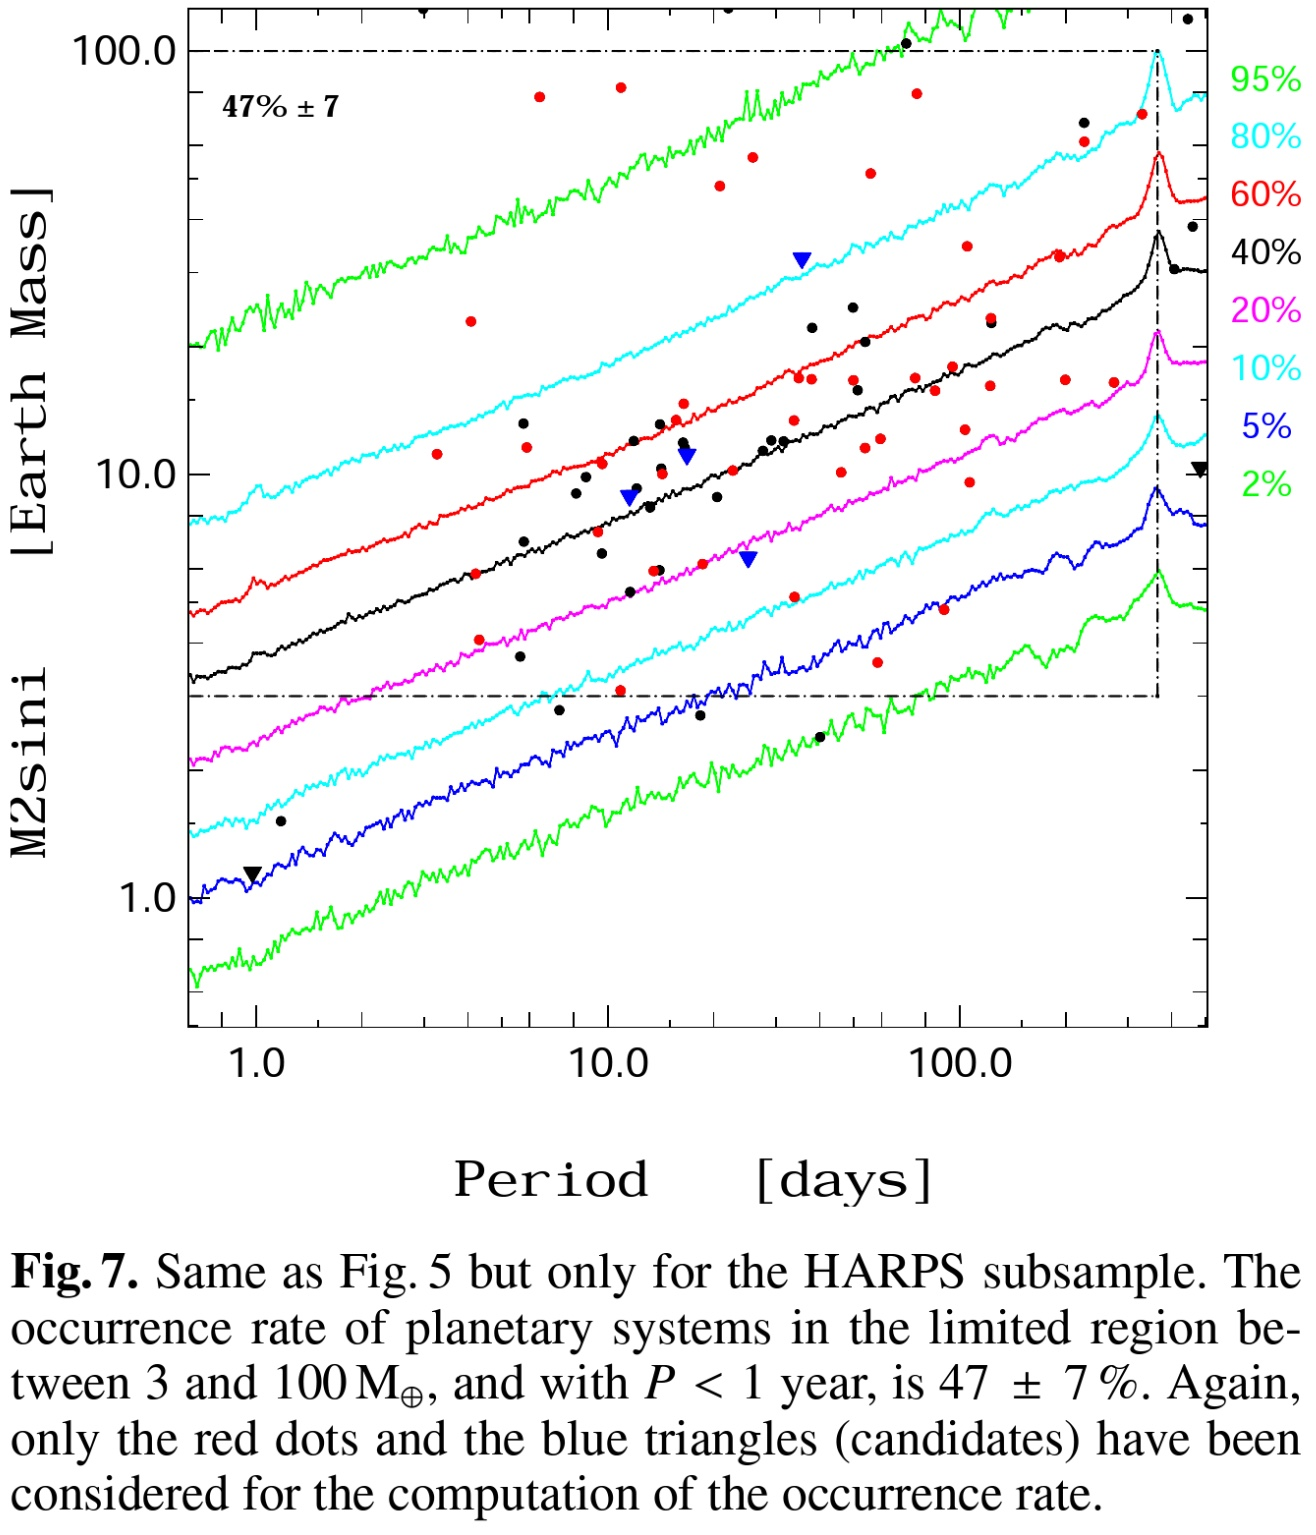
\includegraphics[trim={0cm 10cm 0 0},clip, width=0.99\textwidth]{PMfreq-e12}\label{fig:PMfreq-e12}
	\end{subfigure}%
	
	\begin{subfigure}[b]{0.38\textwidth}
		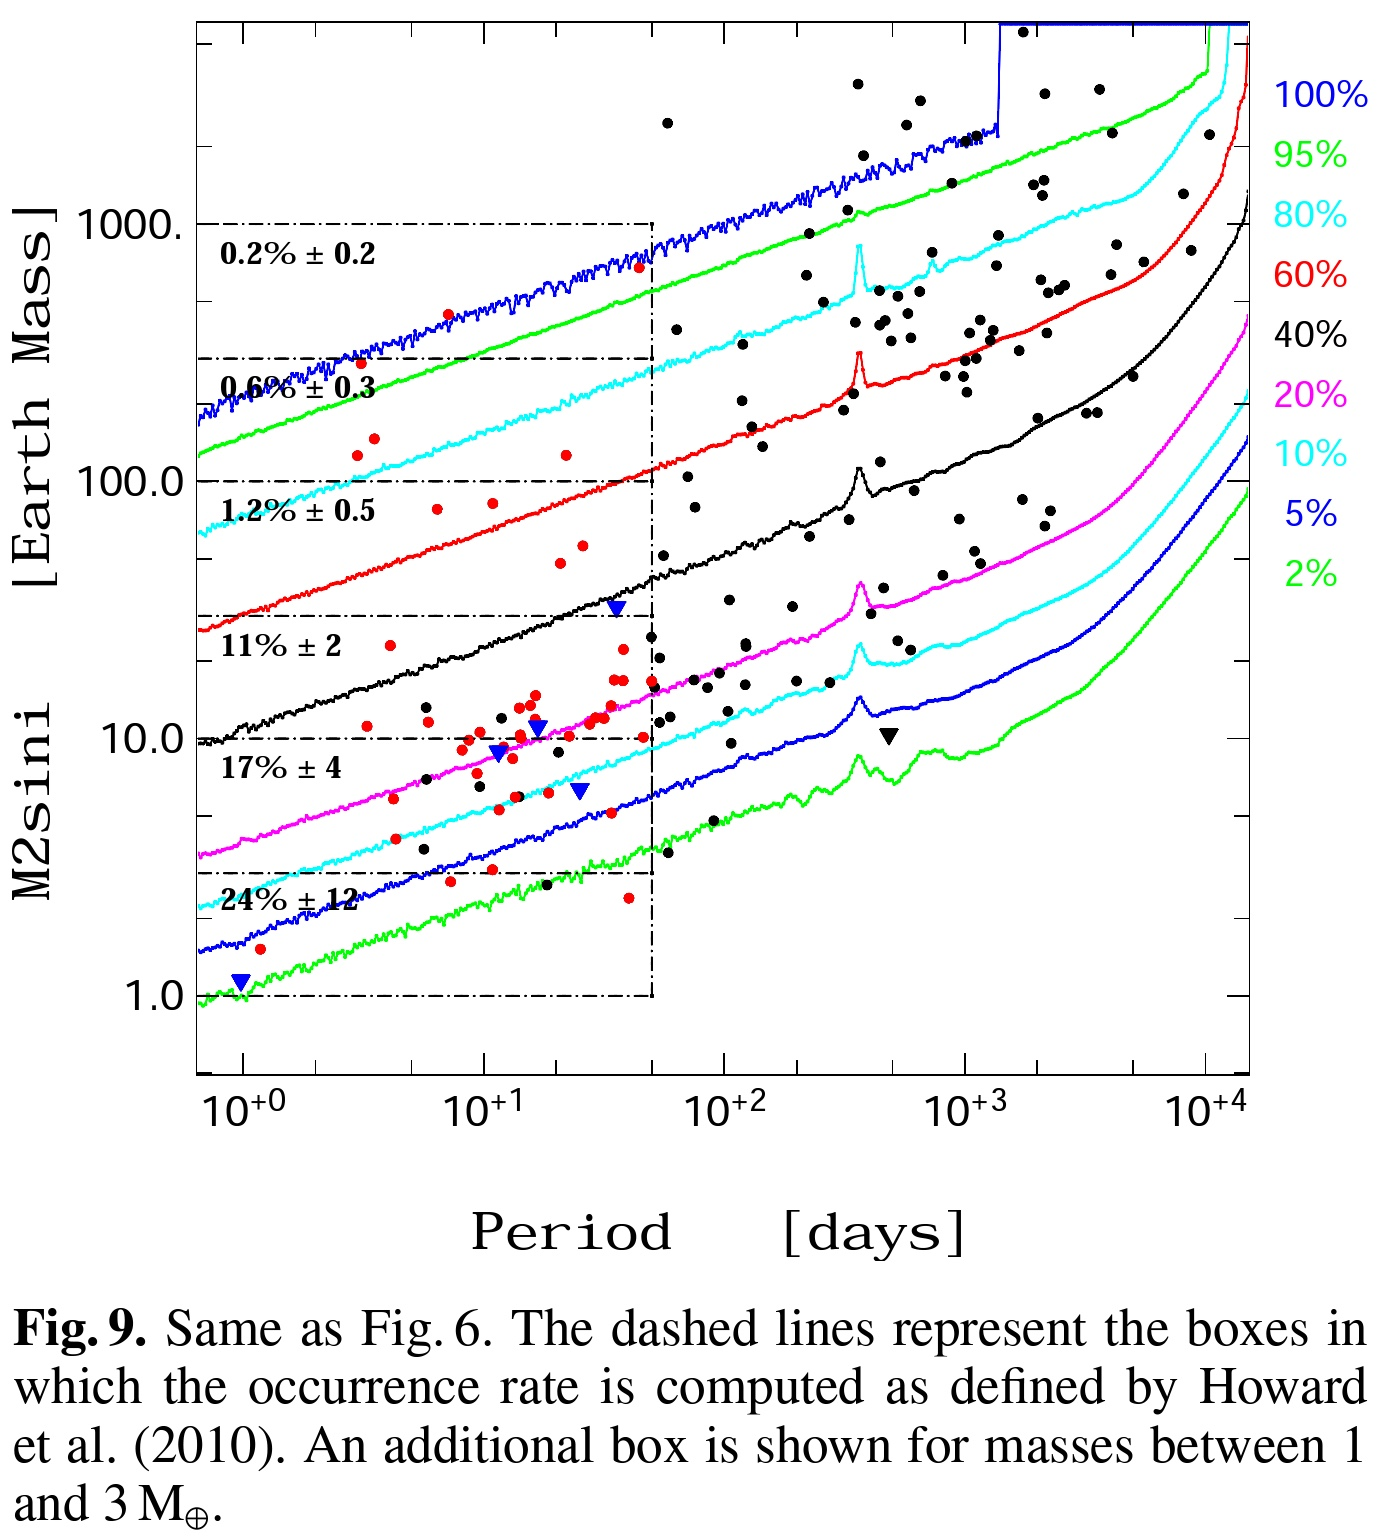
\includegraphics[trim={0cm 8cm 0 0},clip, width=0.99\textwidth]{PMfreq-short}\label{fig:PMfreq-short}
	\end{subfigure}
	\caption{Diagramma massa-periodo: frazione di stelle che ospitano pianeta con caratteristiche nella regione evidenziata. Da sinistra a destra: $P<10\si{\year}$ e $M>50\mearth{}$, $P<1\si{\year}$ e $M>3-100\mearth{}$, $P<50\si{\day}$ e $M=1-3/3-10/10-30/30-100/100-300/300-1000$. Da \cite{mayor2011harps}.}\label{fig:PMfreqs}
\end{figure}
\end{frame}

\begin{wordonframe}{RV survey: frequenze pianeti e bias osservativi}
Adesso passo a descrivere le propriet\'a degli esopianeti: una popolazione numerosa \'e stata osservata tramite osservazione della velocit\'a radiale della stella madre in una survey di 8 anni con lo spettrografo HARPS.
L'ampiezza della velocit\'a con cui la stella si muove \'e determinata dal periodo ($P$) e dalla massa del pianeta ($M_P$) oltre a fattori geometrici. (For Jupiter around the Sun ($a_J=5.2AU$, $P=11.9yr$: $K_J=\SI{12.5}{\meter\per\second}$))
Per tenere sotto controllo i bias osservativi si \'e scelto di fissare la probabilit\'a di rivelamento al $99\%$ e restringersi alle stelle che soddisfano la richiesta nella data regione del diagramma massa-distanza.
Le principali propriet\'a osservate sono massa del pianeta e periodo.
Pianeti gassosi con $M_P>50\mearth{}$, $P<\SI{10}{\year}$: $14\%$.
Pianeti gassosi con $100\mearth{}M_P>3\mearth{}$, $P<\SI{1}{\year}$: $47\%$.
Sistemi copatti con $P<\SI{50}{\day}$ e $M=1-3/3-10/10-30/30-100/100-300/300-1000$


Survey HARPS: radial velocity. La stella percorre ellisse attorno al CM stella-pianeta.
\begin{align*}
&v_r=\dot{z}=K[\cos{(\omega+\nu)}+e\cos{\omega}]\\
&K=\frac{2\pi}{P}\frac{a_*\sin{i}}{(1-e^2)\expy{1/2}}=(\frac{2\pi G}{P})\expy{1/3}\frac{M_p\sin{i}}{(M_p+M_*)\expy{2/3}}\frac{1}{(1-e^2)\expy{1/2}}
\end{align*}
$99\%$ detection threshold: $C(P,m\sin{i})$ frazione di stelle con sufficienti osservazioni per rivelare o escludere pianeta in data regione diagramma $(P,M)$, $N_{ij}=\frac{1}{C(P,M\sin{i})}$.
\end{wordonframe}

\begin{wordonframe}{Terza legge di Keplero}
	\begin{columns}[c]\begin{column}{0.7\textwidth}
			\begin{align*}
			&\ddvec{r}_1-\ddvec{r}_2=-\frac{G(m_1+m_2)}{|\vec{r}_1-\vec{r}_2|^3}(\vec{r}_1-\vec{r}_2)
			\end{align*}
		\end{column} \begin{column}{0.3\textwidth}
			\begin{align*}
			&P^2=\frac{4\pi^2}{G(m_1+m_2)}a^3
			\end{align*}
	\end{column}  \end{columns}
	\begin{columns}[c]\begin{column}{0.7\textwidth}
			\begin{align*}
			&m_1\vec{r}_1+m_2\vec{r}_2=0\\
			&\vec{r}_1-\vec{r}_2=\frac{m_1+m_2}{m_2}\vec{r}_1=-\frac{m_2+m_1}{m_1}\vec{r}_2\\
			&m_1\ddvec{r}_1=-Gm_1m_2\frac{m_2^3}{(m_1+m_2)^3r_1^3}\frac{m_1+m_2}{m_2}\vec{r}_1\\
			&\ddvec{r}_1=-\frac{\mu_1}{r_1^3}\vec{r}_1\\
			&\ddvec{r}_2=-\frac{\mu_2}{r_2^3}\vec{r}_2
			\end{align*}
		\end{column} \begin{column}{0.3\textwidth}
			\begin{align*}
			&P^2=\frac{4\pi^2}{\mu_1}a_1^3\\
			&P^2=\frac{4\pi^2}{\mu_2}a_2^3
			\end{align*}
	\end{column}  \end{columns}
\end{wordonframe}

\begin{frame}{HARPS: Distribuzione metallicit\'a}
\begin{figure}[!ht]
	\centering 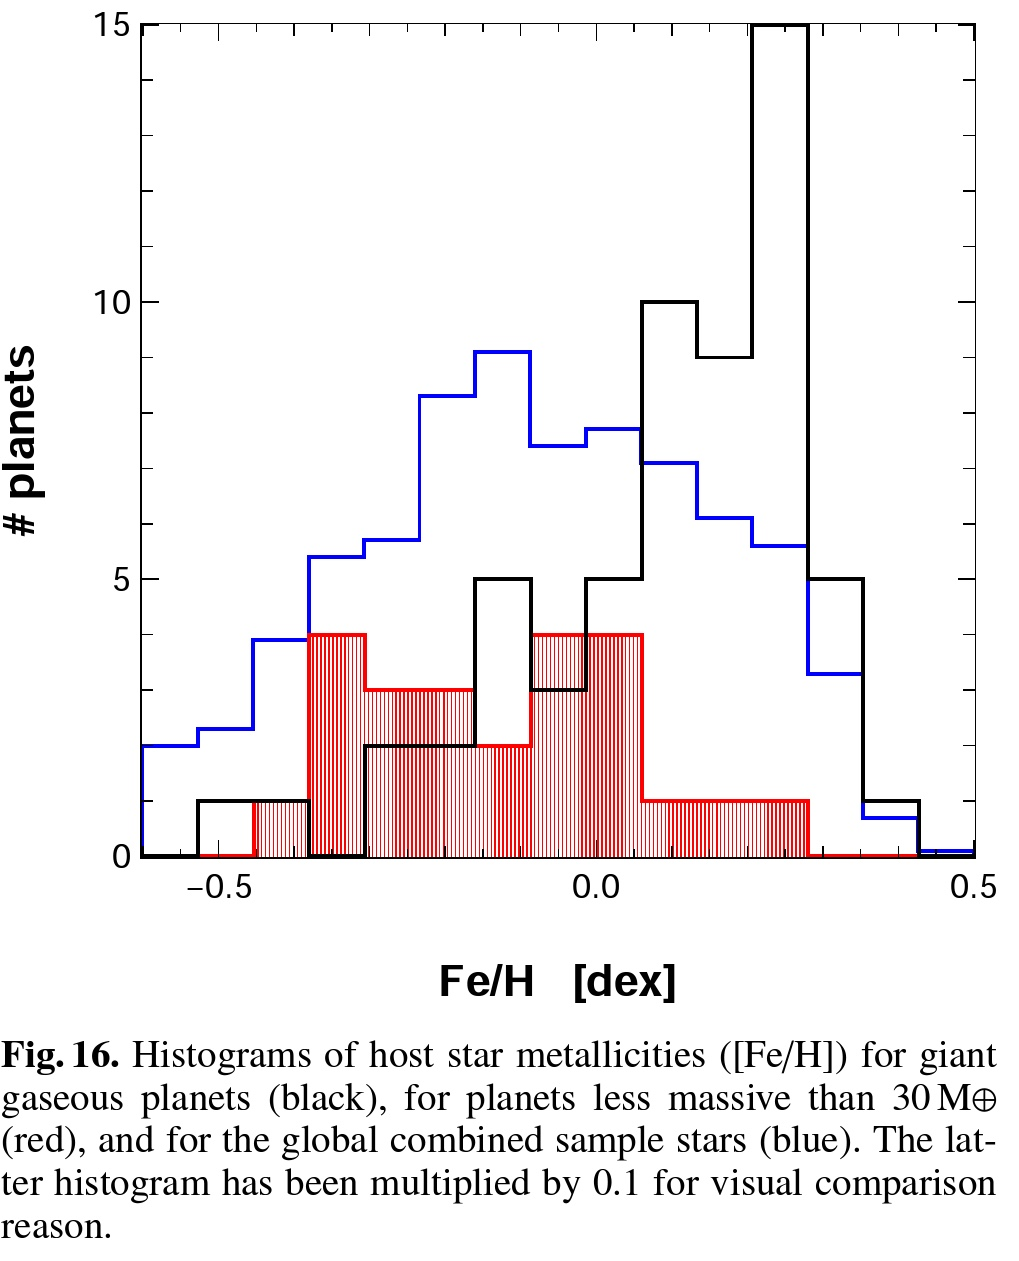
\includegraphics[trim={0cm 8cm 0 0},clip, width=0.53\textwidth]{PfreqvsFeH}
	\caption{Numero di pianeti in funzione della metallicit\'a stellare: nero dei giganti gassosi, rosso dei pianeti con $M\leq30\mearth{}$ e blu combinata. Da \cite{mayor2011harps}.}\label{fig:PfreqvsFeH}
\end{figure}
\end{frame}

\begin{wordonframe}{Harps: metallicit\'a-frequenza pianeti giganti}
La distribuzione dei pianeti con $M\geq30\mearth{}$ cresce con metallicit\'a stellare: il plot nero rappresenta il numero dei pianeti giganti ed \'e correlato con la metallicit\'a della stella.
Questa correlazione pu\'o apparire ovvia nello scenario di core accretion nel senso che maggiore metallicit\'a pu\'o portare prima a raggiungere la massa critica per accrescimento di gas.
\end{wordonframe}

\begin{frame}{HARPS: Distribuzione massa e periodo}
\begin{figure}[!ht]
	\begin{subfigure}[b]{0.45\textwidth} \centering 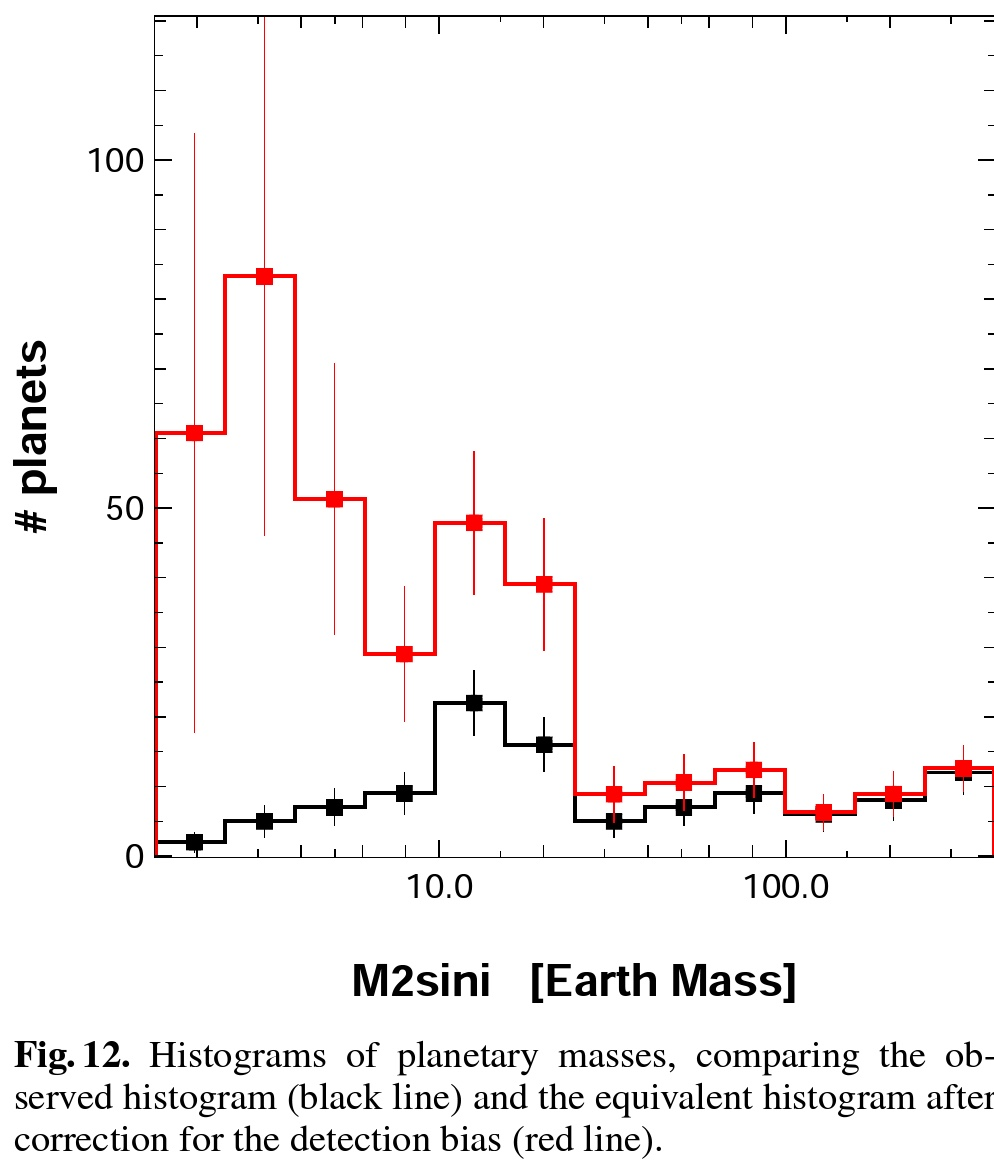
\includegraphics[trim={0cm 5cm 0 0},clip, width=0.94\textwidth]{freqvsM}
		\caption{Distribuzione di massa di massa dei pianeti: in rosso distribuzione corretta per bias osservativi. Da \cite{mayor2011harps}.}\label{fig:freqvsM} \end{subfigure}
	~
	\begin{subfigure}[b]{0.45\textwidth} \centering 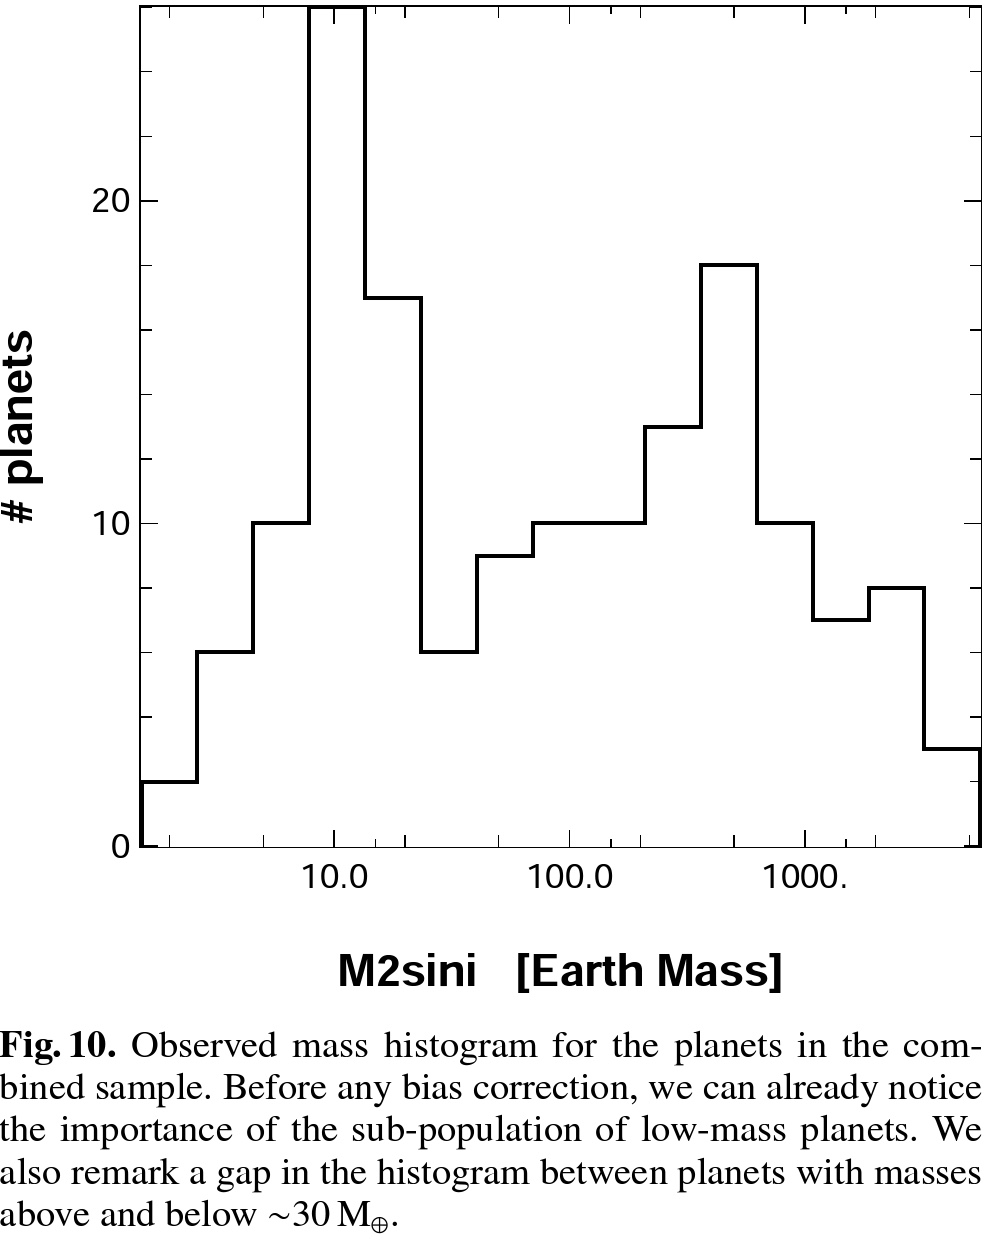
\includegraphics[trim={0cm 8cm 0 0},clip, width=0.94\textwidth]{freqvsMcomb}
		\caption{Distribuzione di massa dei pianeti osservata. Da \cite{mayor2011harps}.}\label{fig:freqvsMcomb}
	\end{subfigure}
\end{figure}
\end{frame}

\begin{wordonframe}{Harps: Distribuzione massa}
Massa: abbondanza pianeti di piccola massa: distribuzione crescente verso piccole masse e rapida diminuzione tra $\num{10}{30}\mearth{}$.
La distribuzione di massa mostra crescita per piccole masse e una rapida discesa tra \numrange{3}{10}$\mearth{}$: come vedremo la massa critica per accrescimento di gas \'e determinata dai modelli di formazione attorno a $10\mearth{}$.
Il picco nel regime dei pianeti giganti potrebbe essere dovuto ai pianeti che hanno accresciuto il gas nella fascia attorno all'orbita: rallentamento dell'accrescimento limitato dall'evoluzione viscosa del disco.
\end{wordonframe}

\begin{frame}{HARPS: Distribuzione periodo}
\begin{figure}[!ht]
\begin{subfigure}[b]{0.45\textwidth} \centering 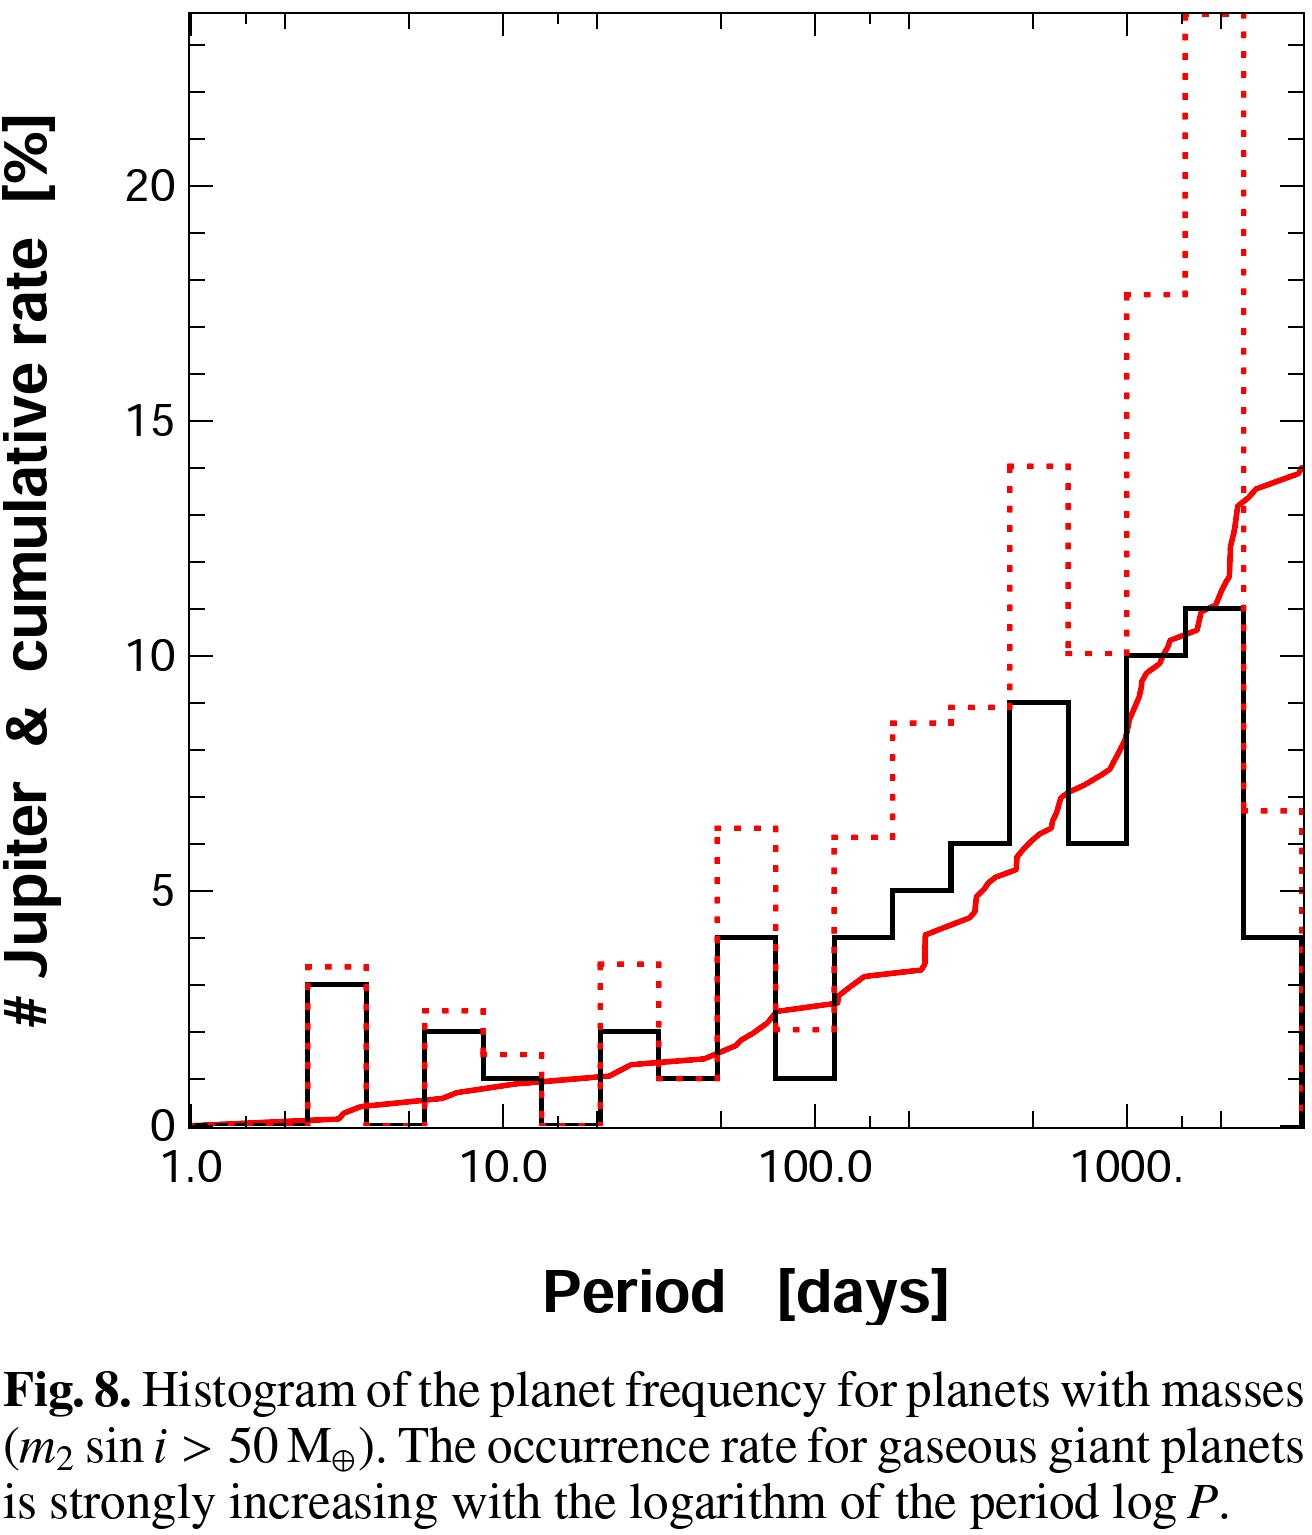
\includegraphics[trim={0cm 6cm 0 0},clip, width=0.98\textwidth]{freqvsPgiant}\caption{Frequenza pianeti con $M\geq 30\mearth{}$ in funzione del periodo orbitale; in rosso  tratteggiato con correzione bias osservativi. Da \cite{mayor2011harps}.}\label{fig:freqvsPgiant} \end{subfigure}
~
\begin{subfigure}[b]{0.45\textwidth} \centering 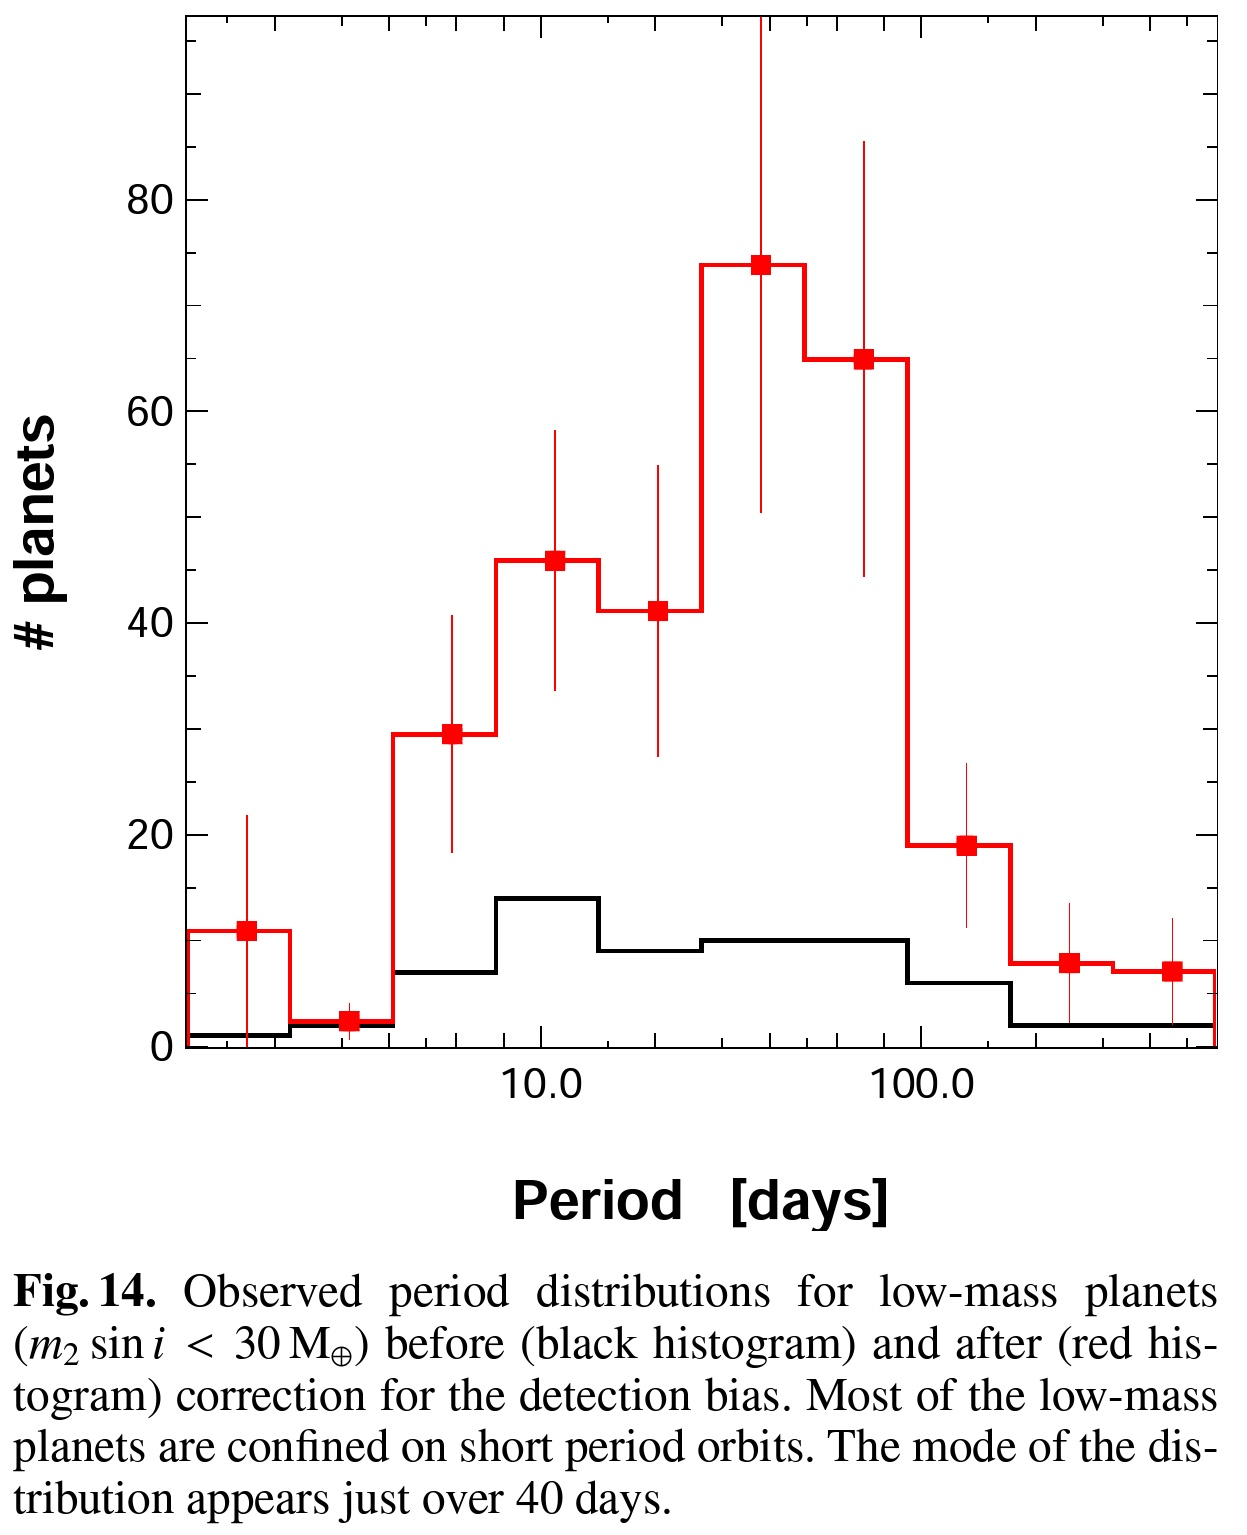
\includegraphics[trim={0cm 10cm 0 0},clip,width=0.98\textwidth]{freqvsPlowM} \caption{Frequenza pianeti con $M\leq 30\mearth{}$ in funzione del periodo orbitale; in rosso con correzione bias osservativi. Da \cite{mayor2011harps}.}\label{fig:freqvsPlowM}
\end{subfigure}
\end{figure}
\end{frame}

\begin{wordonframe}{Harps: Distribuzione periodo}
PAssiamo alla distribuzione dei periodi dove sono distinti i pianeti giganti $M_P>30\mearth{}$ e pianeti con $M_P<30\mearth{}$.
La frequenza dei pianeti giganti cresce con periodo fino a $P=\SI{1000}{\day}$. Pianeti di $M\leq30\mearth{}$ sono concentrati in sistemi compatti con $P=\SIrange{10}{100}{\day}$
\end{wordonframe}

\begin{frame}{Survey: kepler}
\begin{figure}[!ht]
	\begin{columns}[T]
\begin{column}{0.65\textwidth}
	\centering 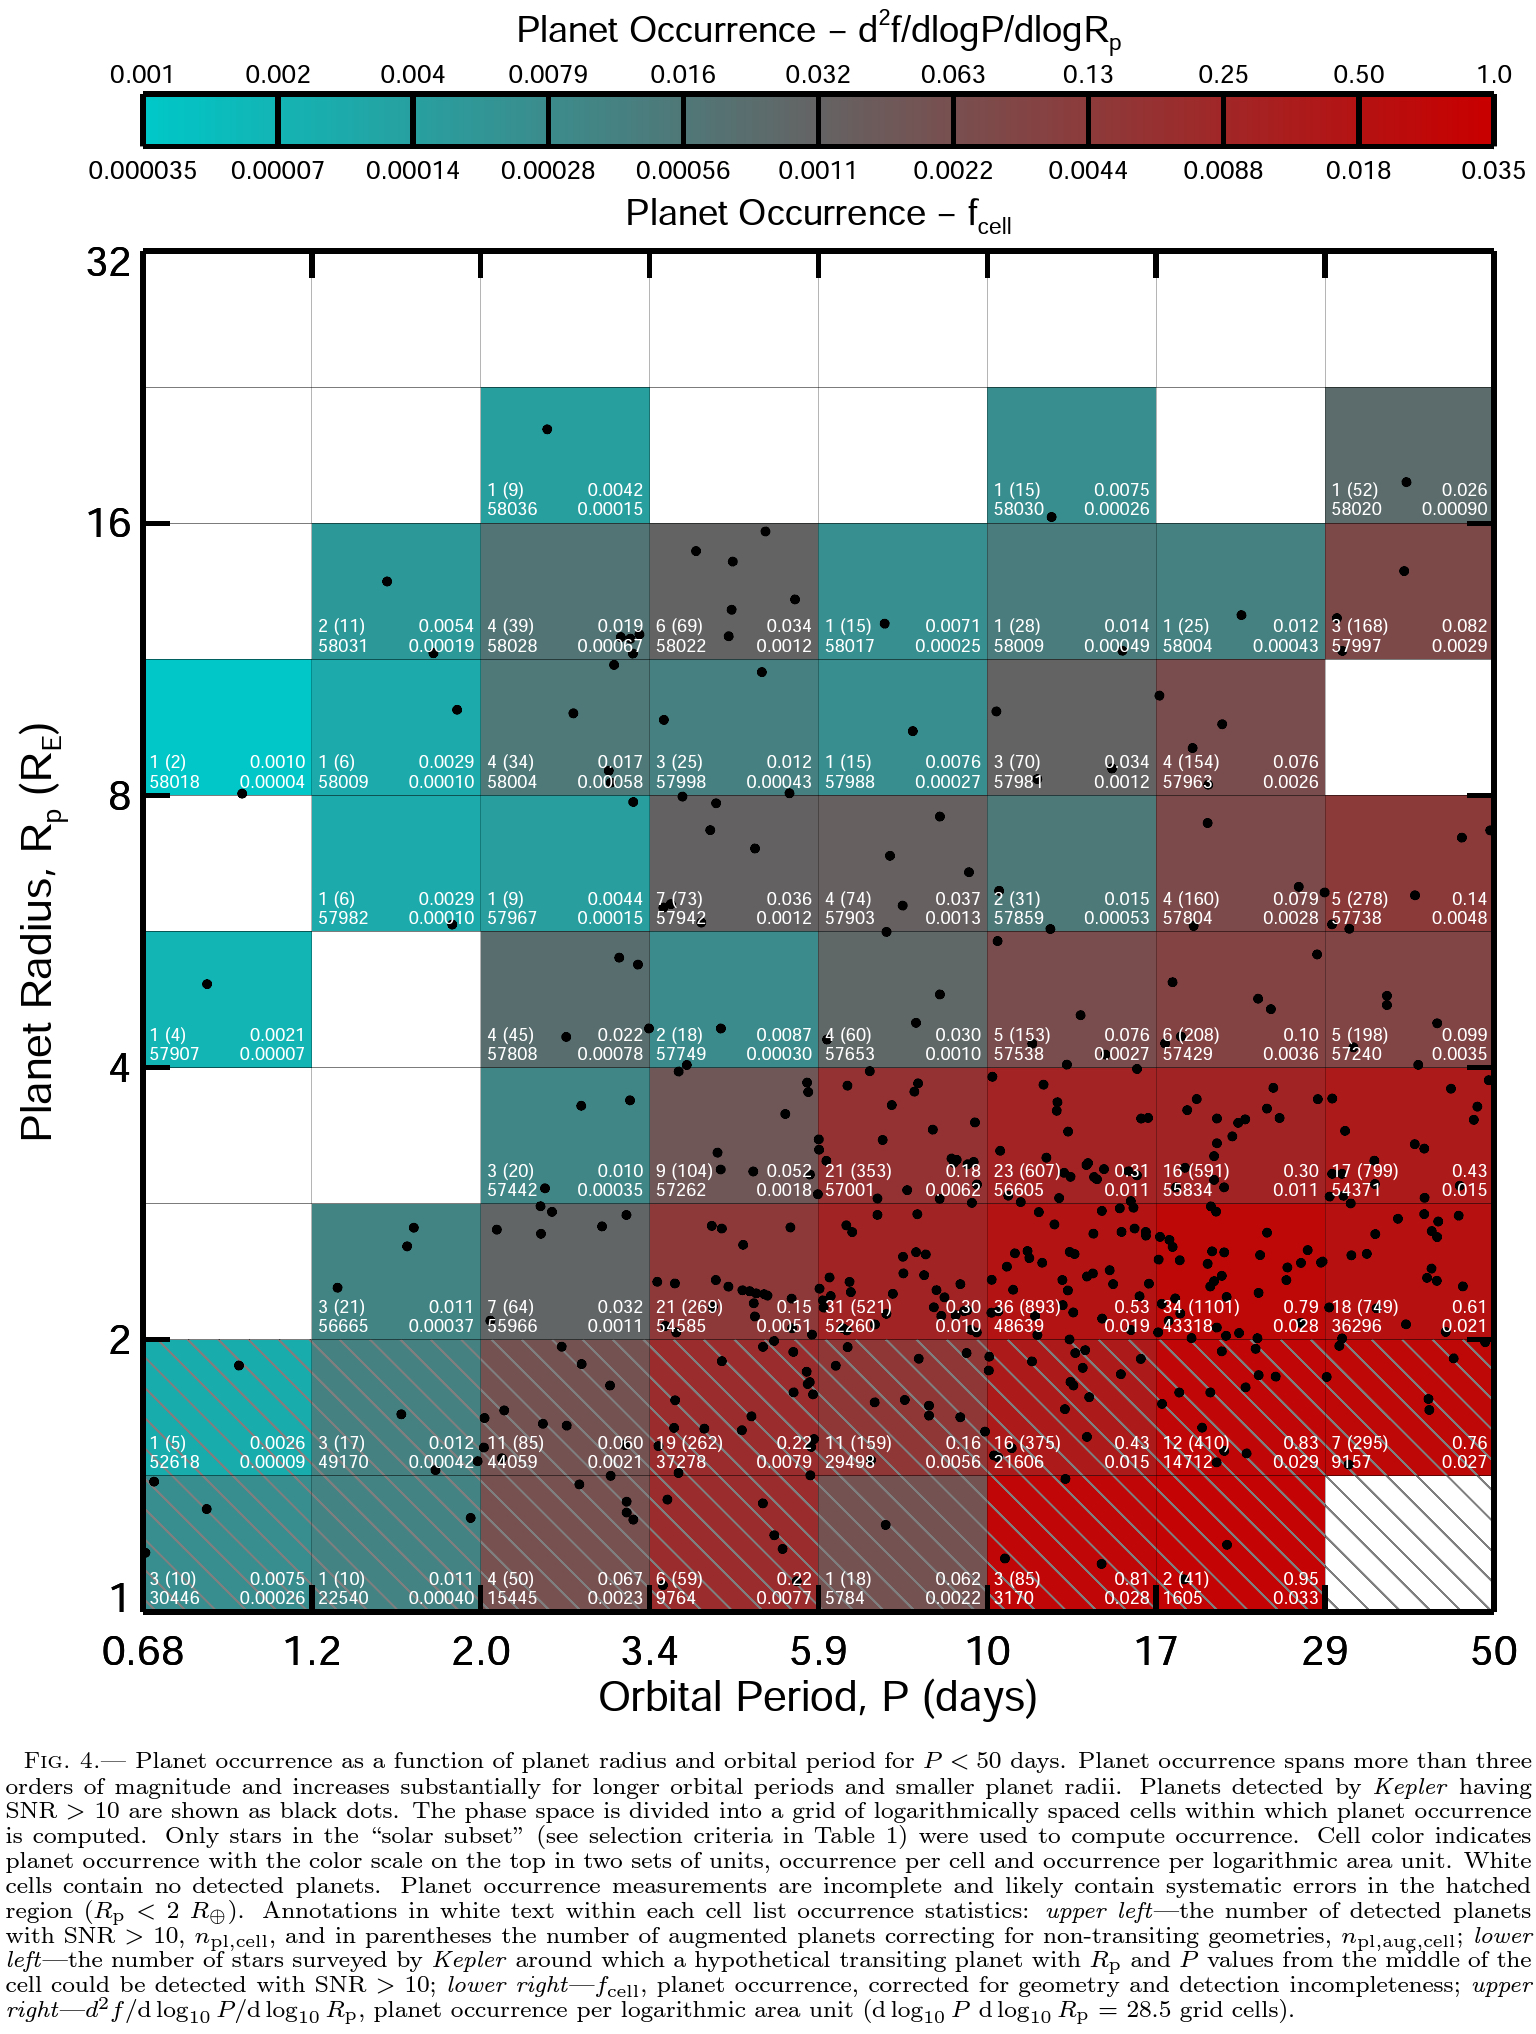
\includegraphics[trim={0cm 11cm 0 0},clip, width=0.9\textwidth]{keplerfreq}
\end{column}
\begin{column}{0.35\textwidth}
\caption{Pianeti con $\SNR{}>10$ nel diagramma $(P,R_P)$. Da \cite{howard2012planet}.}\label{fig:keplerfreq}
\end{column}
	\end{columns}

\end{figure}
\end{frame}

\begin{wordonframe}{Survey: kepler}
Un'altra tecnica osservativa che ha prodotto un abbondanti rivelamenti di pianeti \'e quella dei transiti. Le osservabili fondamentali sono la profondit\'a del transito $\Delta F\approx (R_P/R_*)^2$,cio'e la differenza relativa tra flusso non eclissato ed eclissato, i tempi di transito e il periodo. La probabilit\'a geometrica di transito \'e $\frac{R_*}{a}$ quindi \'e possibile osservare pianeti vicini alla stella. Ho considerato brevemente i risultati della survey eseguita con kepler di cui vediamo i risultati nel diagramma periodo-raggio.
Gli autori dimostrano la completezza delle osservazioni per pianeti con $P<\SI{50}{\day}$ (survey di 90 giorni) e $R_P<50\rearth{}$. In alto a sinistra in ogni cella sono riportati numero di pianeti osservati e la correzione per geometria di transito; mentre in alto a destra occorrenza di pianeti per unit\'a di area logaritmica.


La probabilit\'a che l'orbita di un pianeta sia allineata con l'osservatore in maniera da avere un transito \'e:
\begin{equation*}
p=(\frac{R_*\pm R_p}{a})(\frac{1}{1-e^2})
\end{equation*}
dove $\pm$ indica inclusione/esclusione di transiti a raso.
La maggiore probabilit\'a di transito per orbite eccentriche \'e compensata approssimativamente dalla minore probabilit\'a di rilevamento per la minor durata del transito.
In forma adimensionale l'equazione precedente si riscrive:
\begin{equation}
p=0.005(\frac{R_*}{\rsun{}})(\frac{a}{1AU})\expy{-1}(\frac{1}{1-e^2})
\end{equation}

$\SNR{}=\frac{\delta}{\sigma}\sqrt{\frac{n_{tr}t_{tr}}{\SI{3}{\hour}}}$
upper-left: $n_{pl,cell}(n_{pl,cell,aug})$, pianeti rivelati con $\SNR{}>10$ e correzione per probabilit\'a geometrica transito. Lower-left: stelle surveyed da kepler per cui un pianeta al centro della cella \'e rivelato con $\SNR{}>10$. Lower-right: $f_{cell}$ frequenza di pianeti corretta per probabilit\'a geometrica e incompletezza rivelamento. Upper-right: planet occurrence per logaritmic area unit.
\end{wordonframe}

\begin{frame}{Transiti: distribuzione raggi planetarii}
\begin{figure}[!ht]
	\begin{subfigure}[b]{0.47\textwidth}
		\centering
		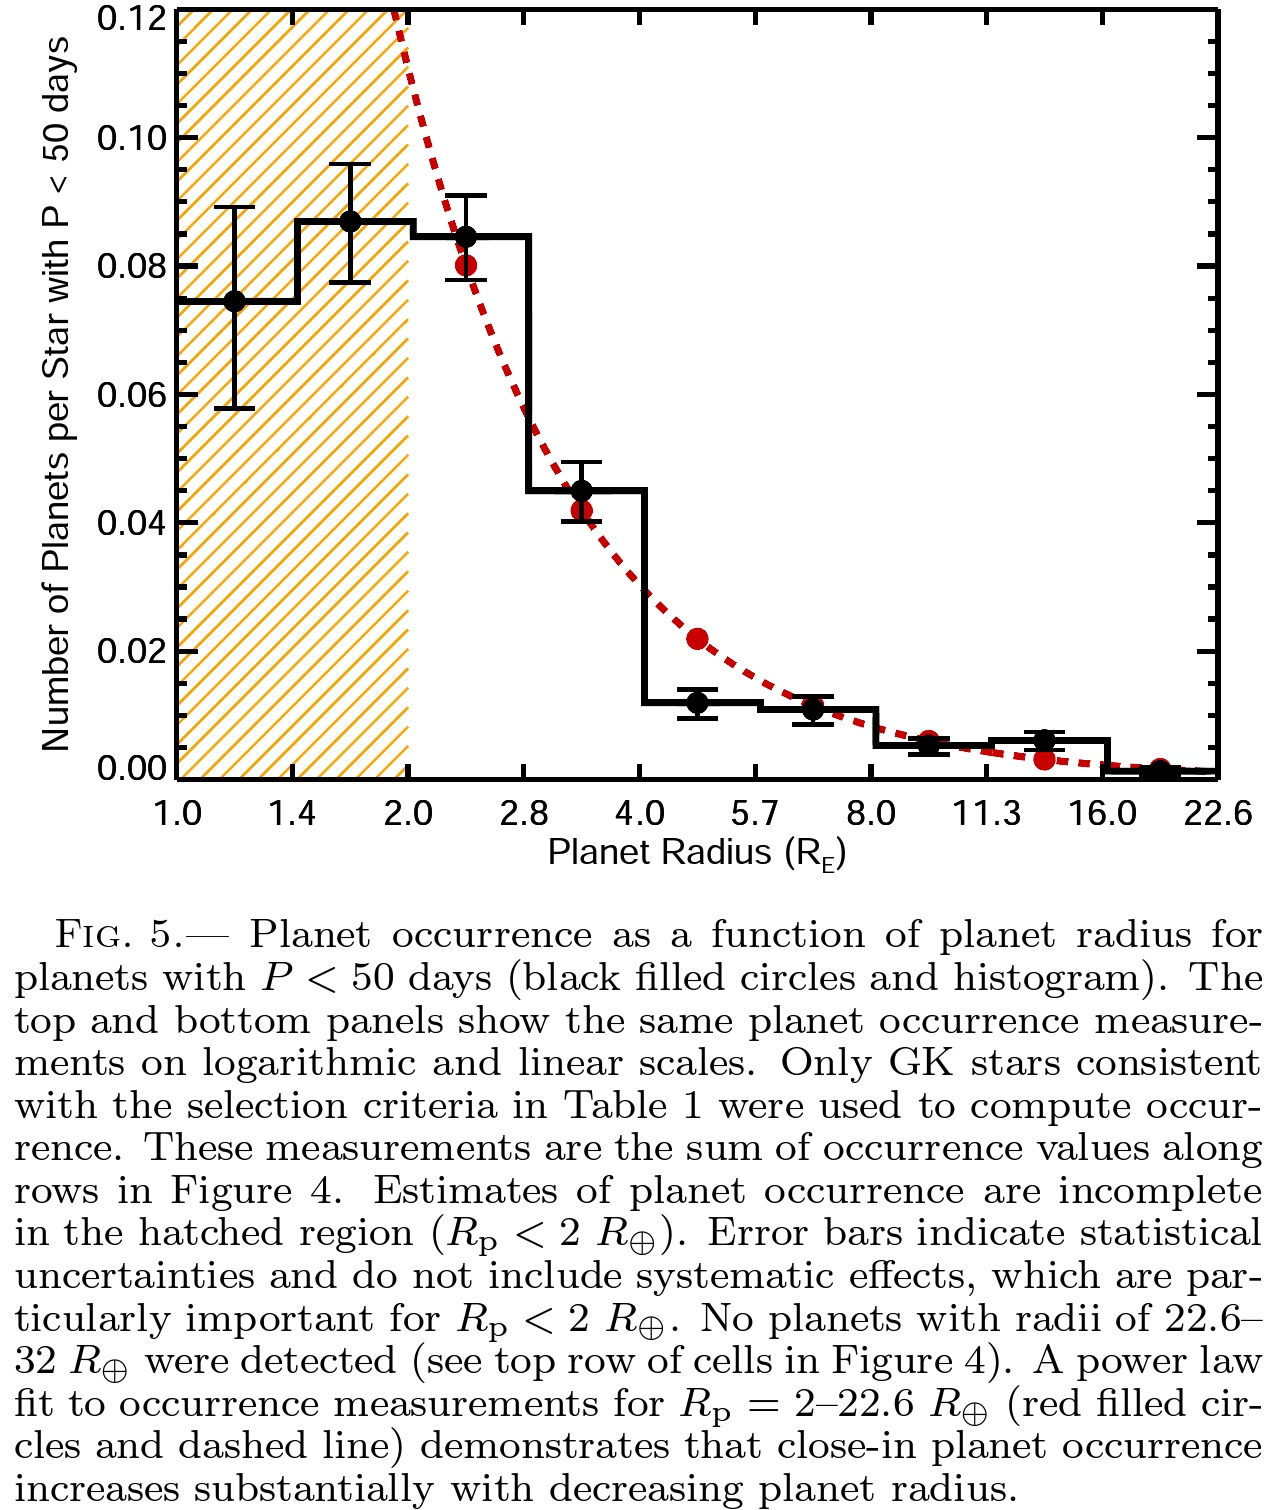
\includegraphics[trim={0cm 22cm 0 0},clip, width=0.95\textwidth]{freqvsRpl50d}
		\caption{Distribuzione raggi planetari: crescita esponenziale verso piccoli raggi. La regione barrata indica misure incomplete. Da \cite{howard2012planet}.}\label{fig:howard2012planet}
	\end{subfigure}
	~
	\begin{subfigure}[b]{0.49\textwidth} \centering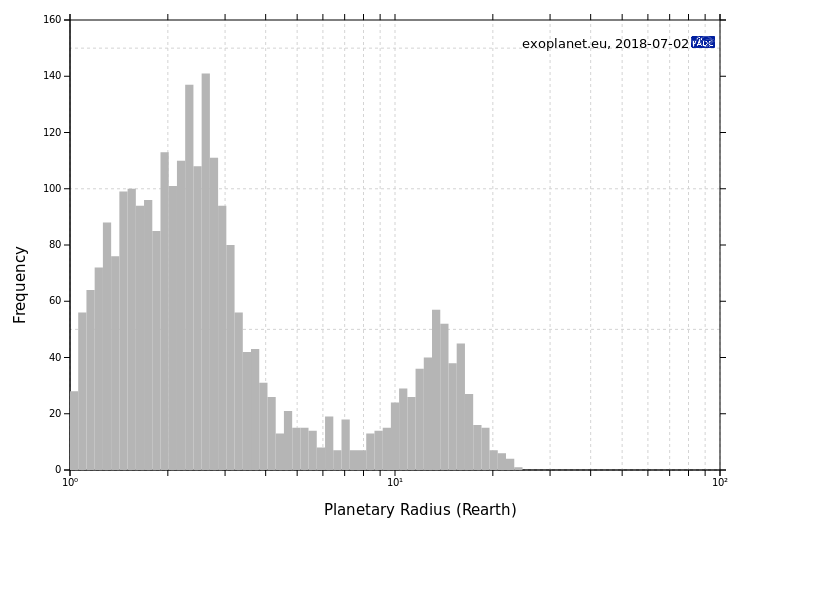
\includegraphics[trim={0cm 2.5cm 0 0},clip, keepaspectratio,width=0.9\textwidth]{Rfreq}\caption{Distribuzione radiale pianeti rivelati tramite T. Da \cite{exoplanet.eu} (luglio 2018): la frequenza ha andamento crescente verso pianeti di raggio terrestre, andamento piatto tra $4-10\rearth{}$ e picco a $R\approx\rjupiter{}$.}\label{fig:Rfreq}
	\end{subfigure}
\end{figure}
\end{frame}

\begin{wordonframe}{T: distribuzione raggi}
Cosa determina la distribuzione dei raggi?

\end{wordonframe}

\begin{frame}{Transiti: distribuzione raggi planetarii}
\begin{figure}[!ht]
	\centering 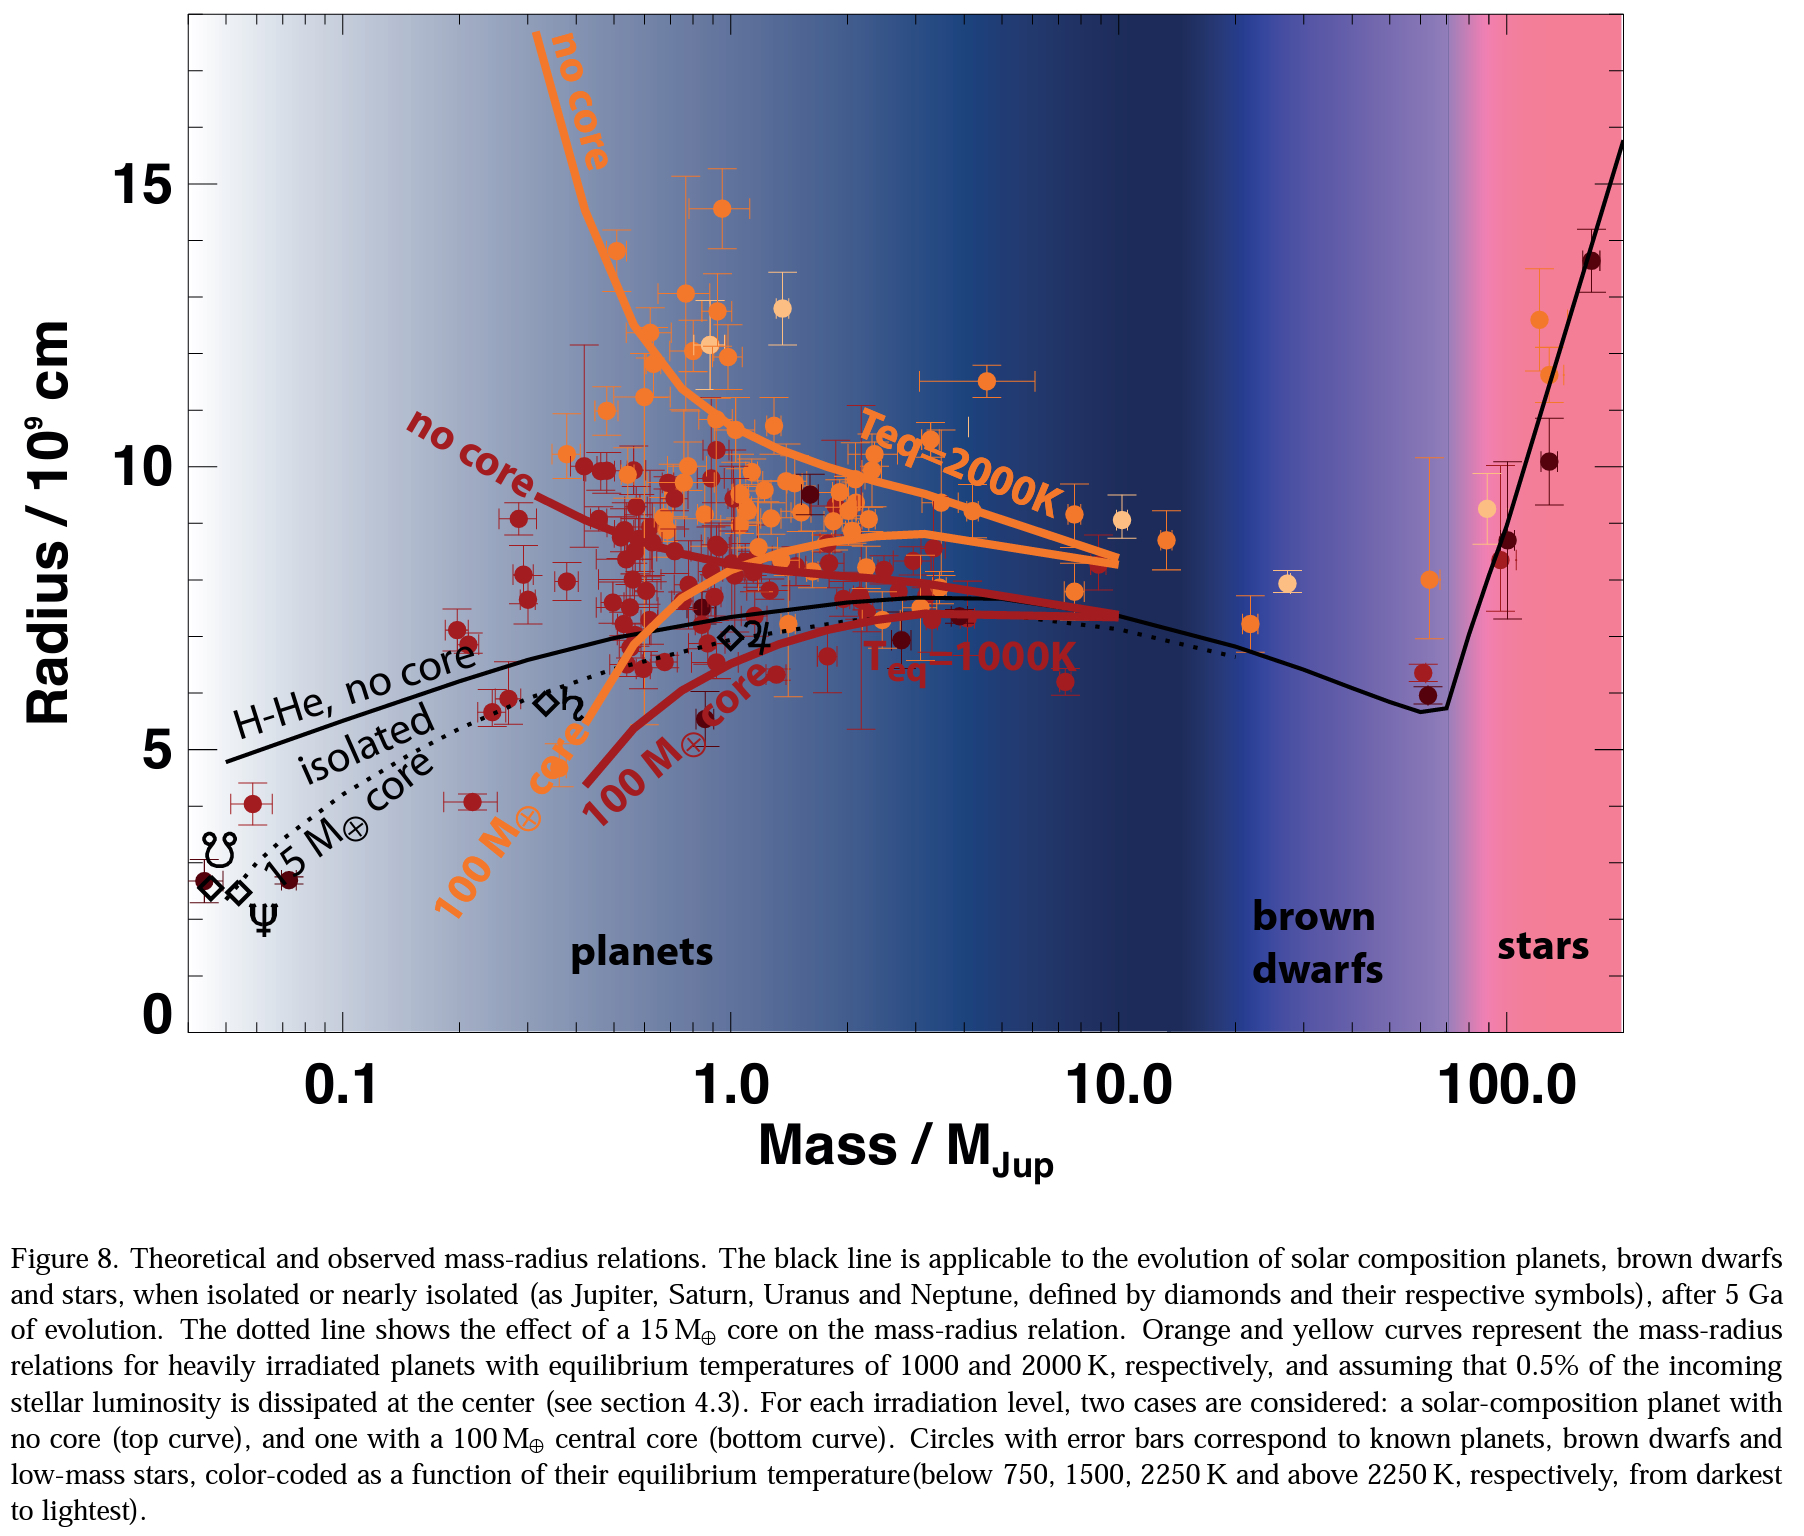
\includegraphics[trim={0cm 12cm 0 0},clip, width=0.8\textwidth]{MR-model-obs}
	\caption{Relazione massa-raggio determinata sulla base di modello planetario dopo \SI{5}{\giga\year}. Per gli esopianeti sono indicate le curve per temperature di equilibrio di \SI{1000}{\kelvin} e \SI{2500}{\kelvin}. Da \cite{guillot2014giant}.}\label{fig:MR-model-obs}
\end{figure}
\end{frame}

\begin{wordonframe}{Relazione massa-raggio}
Determino massa e raggio.
Relazione massa-raggio: 
La determinazione del raggio e massa permette di determinare la densit\'a media del pianeta.
La relazione massa-raggio dipende dalla composizione, che influenza la densit\'a e dall'equazione di stato che determina propriet\'a materia a alte pressioni (compressibilit\'a) e bilancio termico.
consiste in $R\propto M\expy{1/3}$ nella parte incompressibile, $R$indipendente da $M$ per raggi gioviani fino al regime tipico della materia degenere $R\propto M\expy{-1/3}$ nella regione delle brown dwarf.
\end{wordonframe}

\part{Modello di formazione planetaria secondo lo scenario di core accretion}\linkdest{coreaccretion}
\begin{frame}{Dischi di accrescimento: }
\begin{figure}[!ht]
	\begin{subfigure}[b]{0.39\textwidth}
		\centering
		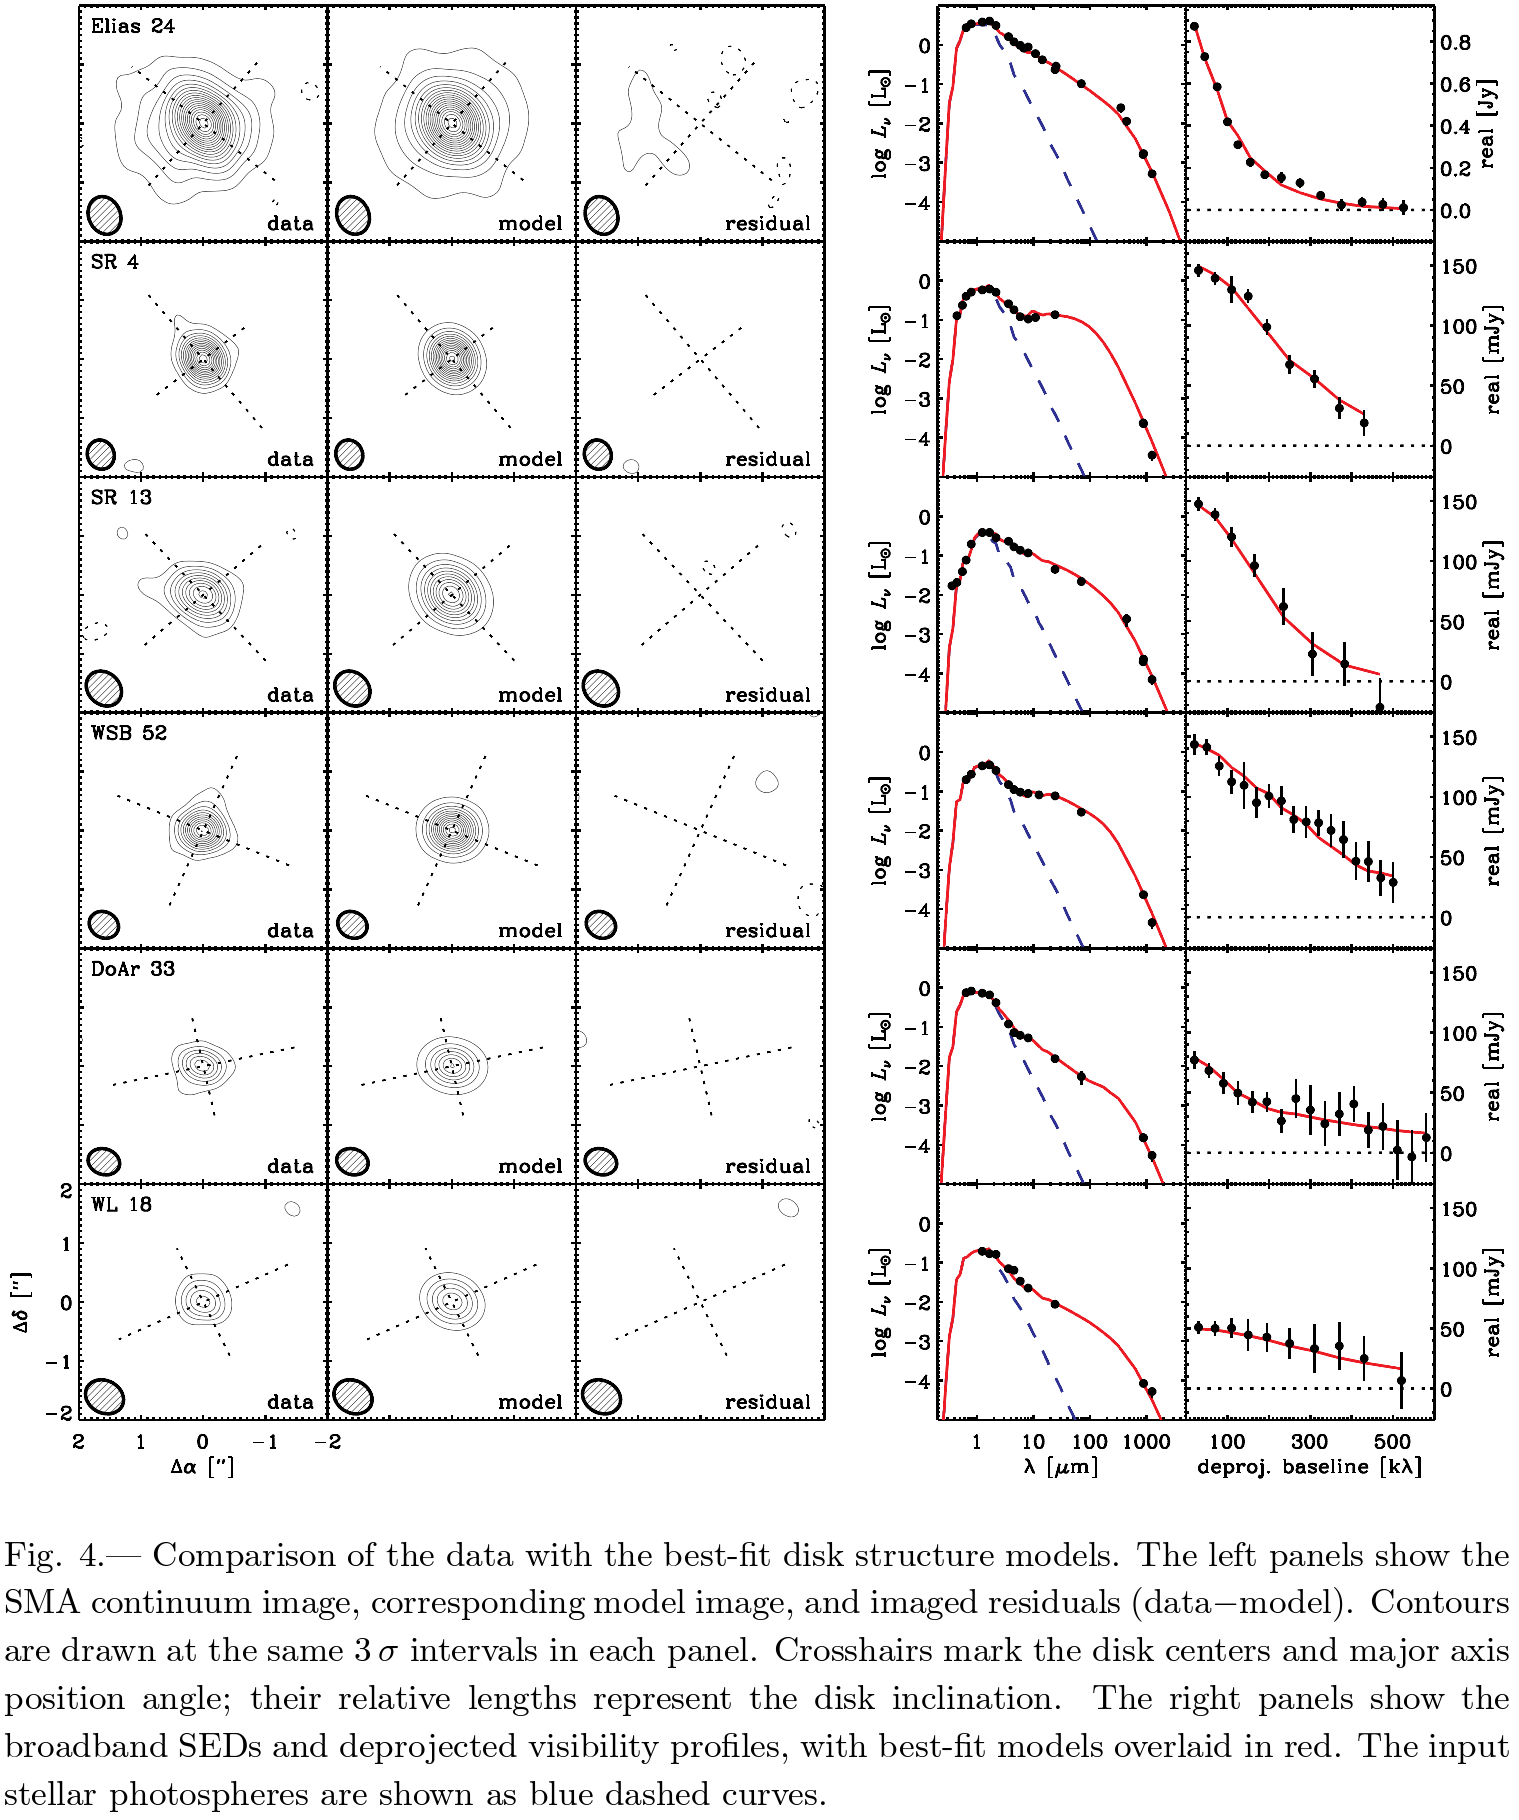
\includegraphics[trim={0cm 10cm 0 0},clip, keepaspectratio,width=0.98\textwidth]{SED-contours}
		\caption{Da \cite{andrews2010protoplanetary}.}\label{fig:SED-contours}
	\end{subfigure}
	~
	\begin{subfigure}[b]{0.55\textwidth}
		\centering
		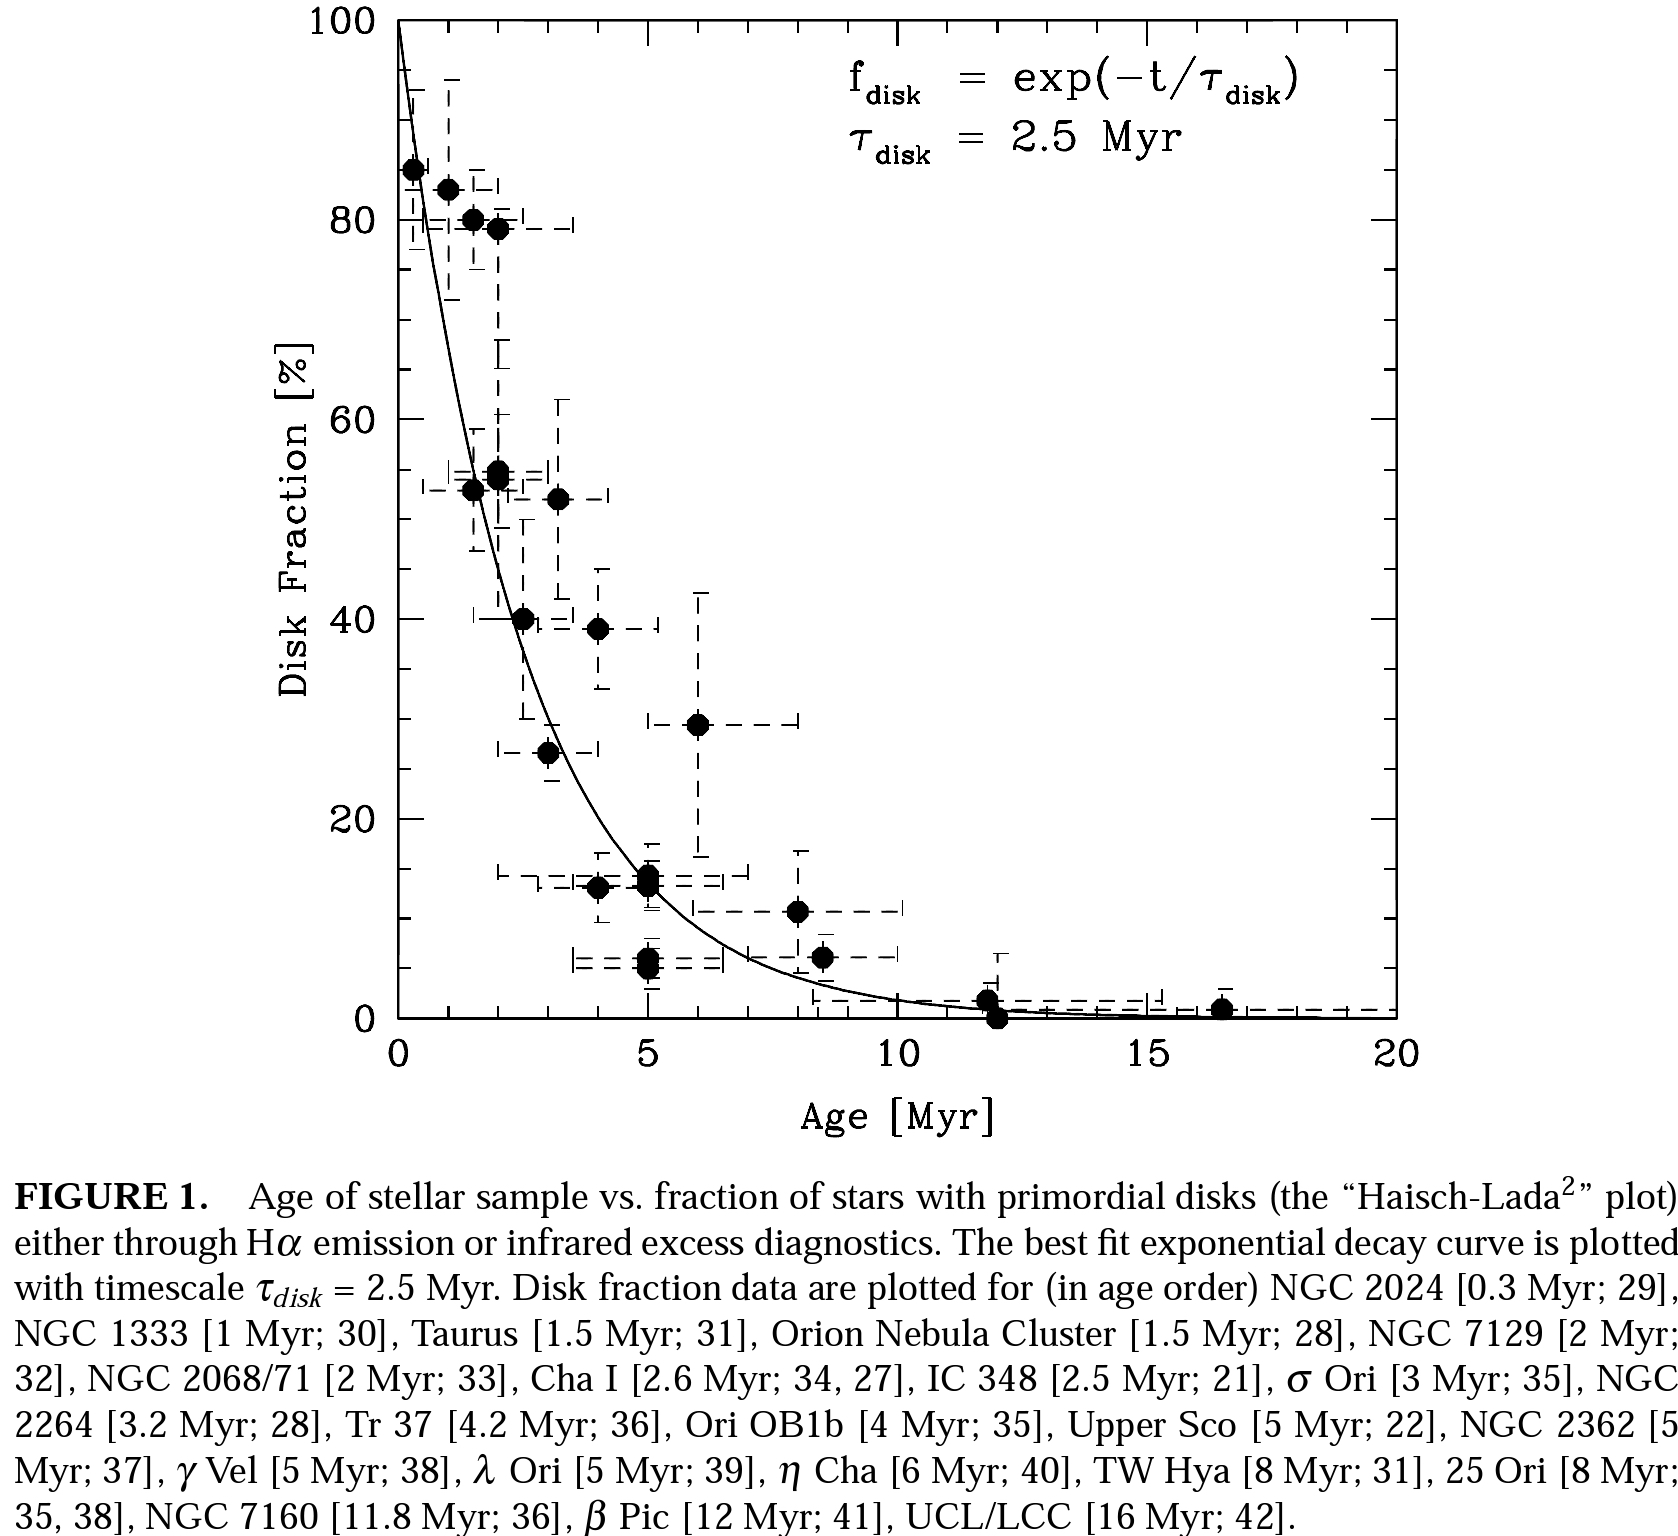
\includegraphics[trim={0cm 13cm 0 0},clip, width=0.99\textwidth,keepaspectratio]{clusterage-fstar}
		\caption{Da \cite{mamajek2009initial}. }\label{fig:clusterage-fstar}
	\end{subfigure}
\end{figure}
\begin{columns}[T]
\begin{column}{0.5\textwidth}
\begin{align*}
&\sigma_{r\phi}=\Sigma\nu r \TDy{r}{\Omega}\\
&\nu=\alpha c_sH
\end{align*}
\end{column}
\begin{column}{0.5\textwidth}
\begin{equation*}
\PDy{t}{\Sigma}=3\frac{1}{r}\PDof{r}[r\expy{1/2}\PDof{r}(\nu\Sigma r\expy{1/2})]\label{eq:sigmaevol}
\end{equation*}
\end{column}
\end{columns}
\end{frame}

\begin{frame}{Evoluzione del disco di polvere. Formazione dei nuclei solidi}

\begin{columns}[T]
\begin{column}{0.37\textwidth}
	\begin{block}{Sedimentazione e drag-forces}
\begin{align*}
&m_p\TDy{t}{\vec{v}}=\vec{F}_D-m_p\Omega^2z\hat{z}\\
&F_D=\frac{1}{2}C_D\pi s^2\rho_gv^2
\end{align*}
\end{block}
\end{column}
\begin{column}{0.63\textwidth}
\begin{block}{Raggiungimento scala chilometrica: planetesimi}
Modello di Goldreich-Ward: disco di polvere sottile instabile.

In assenza di sedimentazione: urti a 2 corpi. Ruolo duplice della turbolenza.
\end{block}
\end{column}
\end{columns}
\begin{block}{Accrescimento protopianeti}
\begin{columns}[T]
\begin{column}{0.5\textwidth}
		\begin{align*}
		&\TDy{t}{M_e}=\pi R_e^2\rho_{pl}v F_g\\
		&=A\pi R_e^2\Sigma_p\Omega F_g
		\end{align*}
\end{column}
\begin{column}{0.5\textwidth}
\begin{align*}
&v\approx\sqrt{e^2+i^2}v_K\\
&f(e,i)=4\frac{\Sigma_p}{m}\frac{ei}{\exv{e^2}\exv{i^2}}\Exp{-\frac{e^2}{\exv{e^2}}-\frac{i^2}{\exv{i^2}}}
\end{align*}
\end{column}
\end{columns}
\end{block}
\end{frame}

\begin{wordonframe}{Disco di polvere e formazione di nuclei solidi: planetesimi}
nel caso cammino libero medio delle molecole di gas sia maggiore delle dimensioni della particella $C_D=\frac{8}{3}\frac{v_{th}}{v_z}$ (Epstein drag) per particelle pi\'u grandi \'e funzione del numero di Reynold.
	dove si assume che eccentricit\'a e inclinazione seguano distribuzione di Rayleigh (\cite{ida1992n})
	$M_{iso}=0.066\mearth{}$ a 1AU densit\'a MMSN $\Sigma_p=\SI{10}{\gram\per\square\cm}$, $M_{iso}=1.36\mearth{}$ a 5AU densit\'a MMSN $\Sigma_p=\SI{3}{\gram\per\square\cm}$,
\end{wordonframe}

\begin{frame}{Fase accrescimento di gas}
\begin{columns}[T]
	\begin{column}{0.5\textwidth}
		\begin{figure}[!ht]
			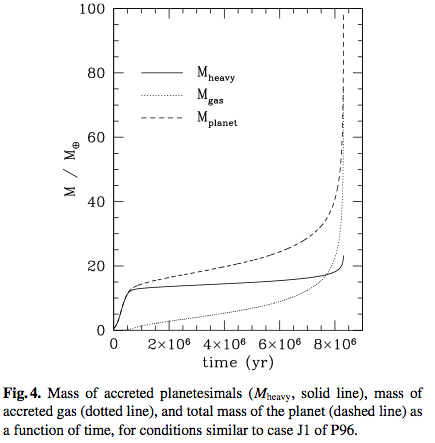
\includegraphics[trim={0cm 2cm 0 0},clip, keepaspectratio,width=0.98\textwidth]{massenvvscore}
			\caption{Da \cite{alibert2005models}.}\label{fig:massenvvscore}
		\end{figure}
	\end{column}
	\begin{column}{0.5\textwidth}
\begin{itemize}
	\item Accrescimento solidi runaway: $\frac{\dot{M}_e}{M_e}\propto M_e\expy{\frac{1}{3}}$
	\item Accrescimento gas su tempo scala $\tkh{}$
	\item Per $M_p\approx7-10\mearth{}$ crescita esponenziale dell'accrescimento di gas
	\item Accrescimento limitato da evoluzione viscosa del disco
\end{itemize}
\end{column}
\end{columns}
\end{frame}

\begin{frame}{Migrazione dei protopianeti}
\begin{columns}[T]
	\begin{column}{0.5\textwidth}
\begin{figure}[!ht]
	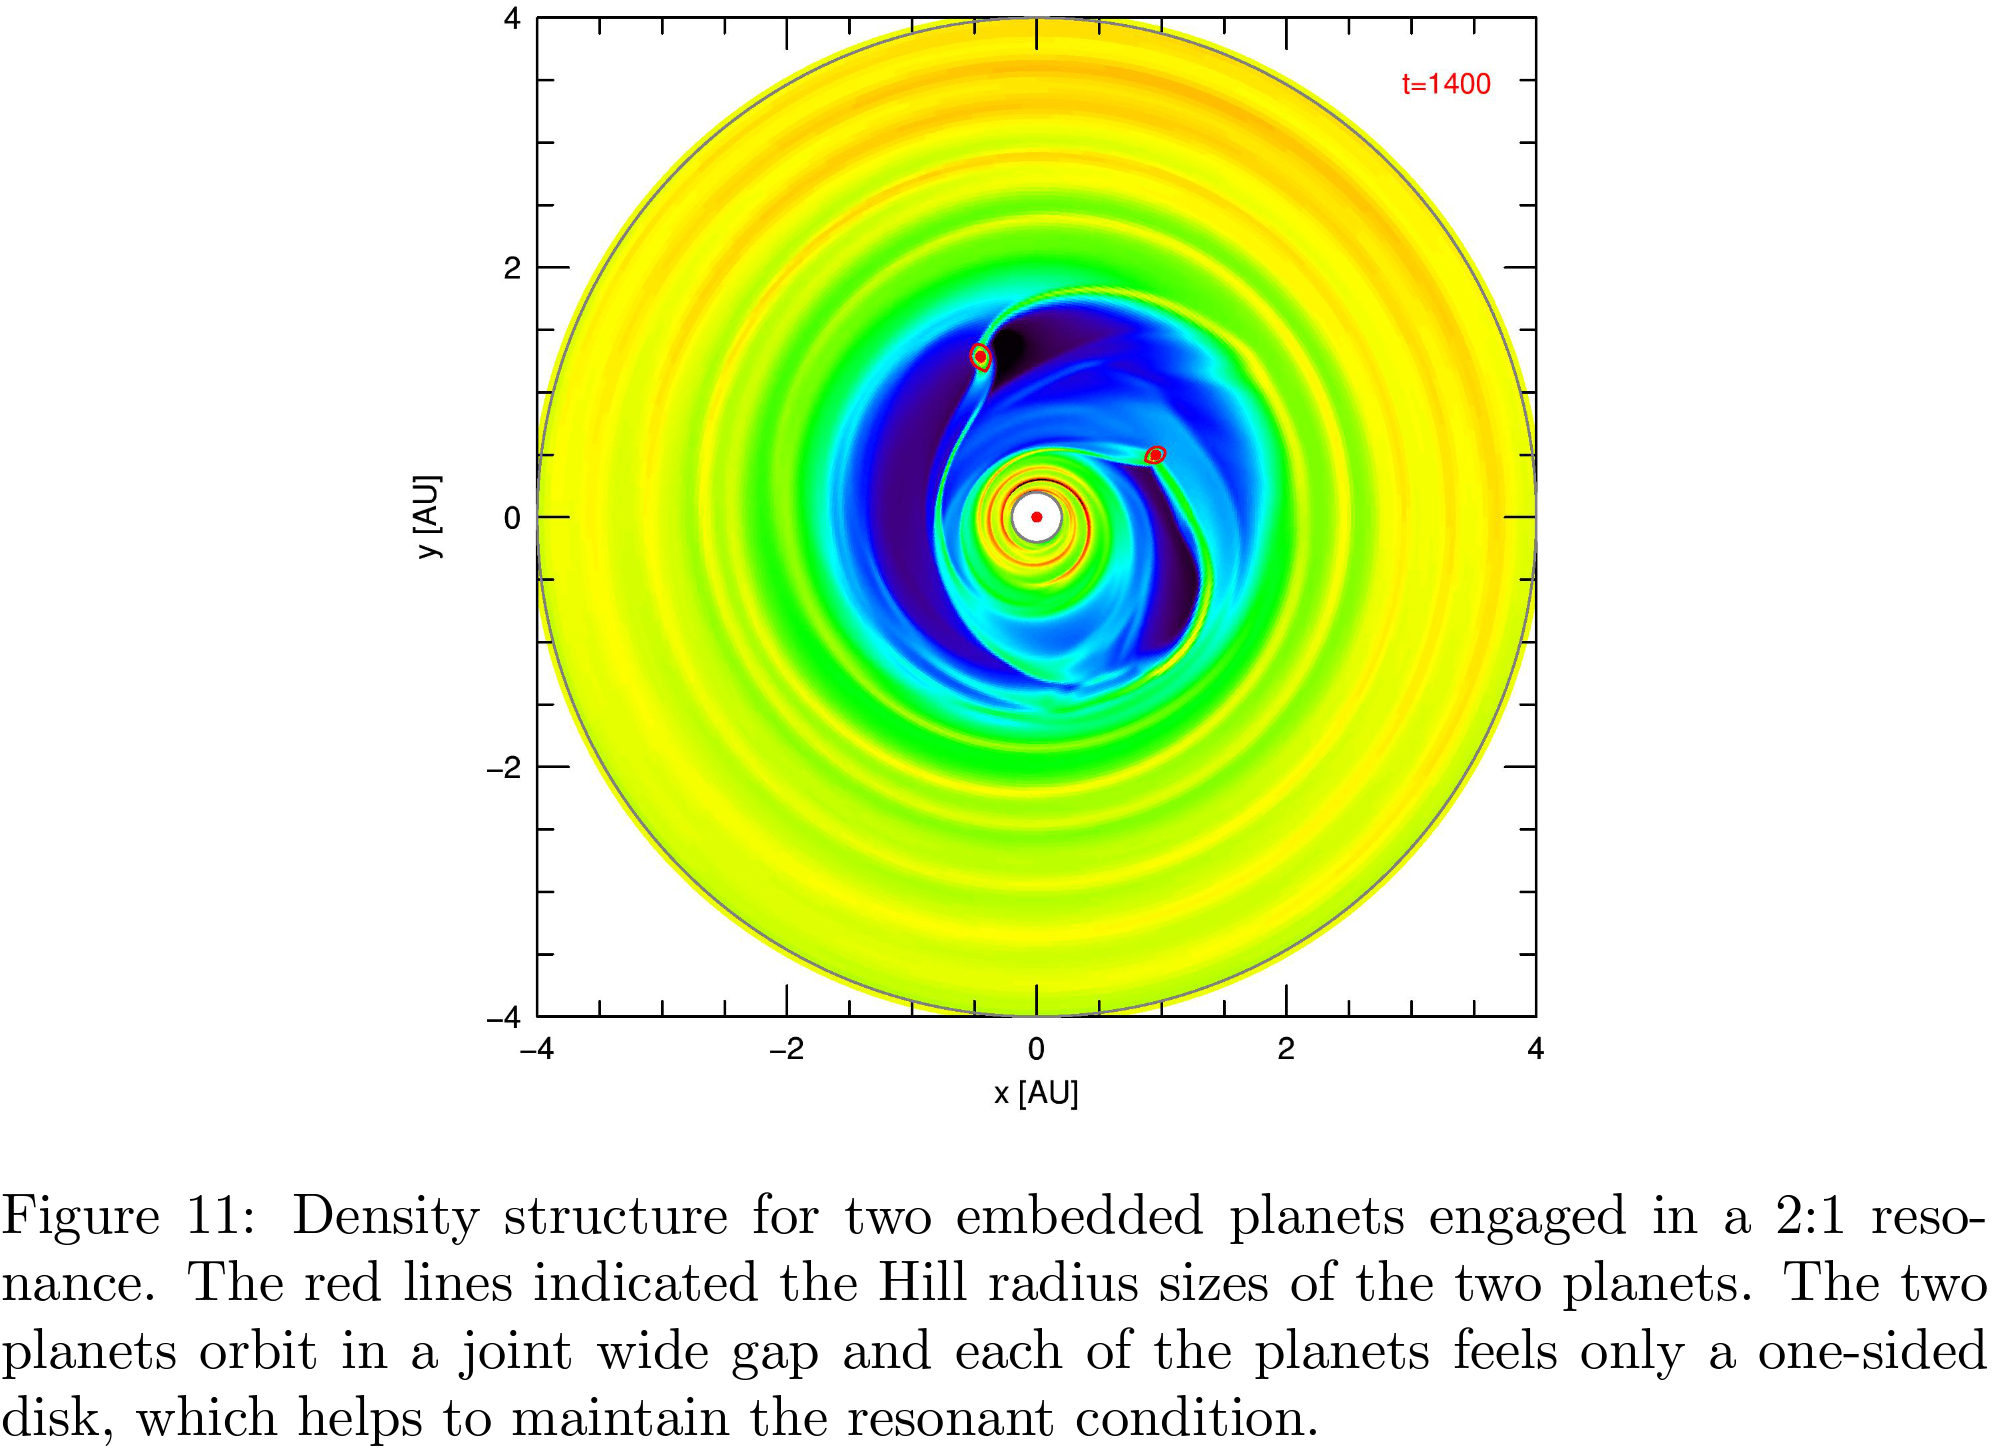
\includegraphics[trim={0cm 11cm 0 0},clip, keepaspectratio,width=0.98\textwidth]{pdres}
	\caption{Simulazione evoluzione orbite planetarie in disco di accrescimento fino a cattura in risonanza $2:1$: le regioni pi\'u dense sono in rosso. Da \cite{kley2012planet}.}\label{fig:pdres}
\end{figure}
	\end{column}
\begin{column}{0.5\textwidth}
\begin{itemize}
	\item Interazione con disco proto-planetario. 
	\item Interazione con disco residuo di planetesimi
	\item Interazione tra due o pi\'u pianeti giganti
	\item Interazione con stella in sistema di stelle binarie
	\item Interazione mareale con la stella
\end{itemize}
\end{column}
\end{columns}
\end{frame}

\begin{wordonframe}{Migrazione planetaria:}
L'osservazione di una sottopopolazione di esopianeti giganti su orbite strette, per cui sembra improbabile una formazione in loco, e la presenza di sistemi multipli in risonanza sono indicatori di evoluzione orbitale, d'altra parte nel Sistema solare fenomeni di migrazione fornisco una spiegazione all'orbita di plutone, alla presenza di numerosi oggetti della fascia di Kuiper in risonanza $3:2$ con Nettuno e al periodo di collisioni intense testimoniato da craterizzazione (Late heavy bombardment).

\end{wordonframe}

\part{Simulazione popolazioni planetarie sintetiche}\linkdest{description}
\section{Modelli di formazione globali. Costruzione popolazioni sintetiche}

\begin{wordonframe}{Popolazione sintetica: Caratteristiche orbitali}
\begin{itemize}
\item Sistemi con solo pianeti di piccola massa ($M_P<10\mearth{}$): bassa densit\'a superficiale di gas e polvere, piccolo tempo di vita del disco ma anche alta metallicit\'a;: scarsa migrazione e interazione dinamica ma evaporazione;
\item Distribuzione piccolo-grosso-piccolo: accrescimento di planetesimi con scarsa migrazione/redistribuzione di solidi; lo sweet point per formazione di pianeti giganti \'e all'esterno dell'iceline
pianeti rocciosi di piccola massa (scarsa componente solida disponibile) all'interno di pianeti giganti, pianeti di ghiacci all'esterno di pianeti giganti (lungo tempo di accrescimento).
Numero di pianeti giganti 1-5: distribuzione di massa varia, pianeta gigante pi\'u interno a circa \SI{1}{\astronmicalunit}; eccentricit\'a \numrange{0}{2}.
\item sistemi ad alta metallicit\'a in cui resta un solo pianeta gigante a seguito di scattering pp ($30\mjupiter{}$, $a_p\approx\SIrange{20}{50}{\astronomicalunit}$)
\item Diagramma a-R a \SI{5}{\giga\year}. $M_e/M_c>1$ $R>6-7\rearth{}$, $M_e/M_c\leq1$ $R>3-4\rearth{}$ uniform in $\log{R}$.
Pianeti giganti in $10-12.4\rearth{}$: non ho considerato variazioni di opacit\'a. Gap dell'evaporazione
\end{itemize}
\end{wordonframe}

\begin{frame}{Modelli di formazione globali}
\begin{figure}[!ht]
	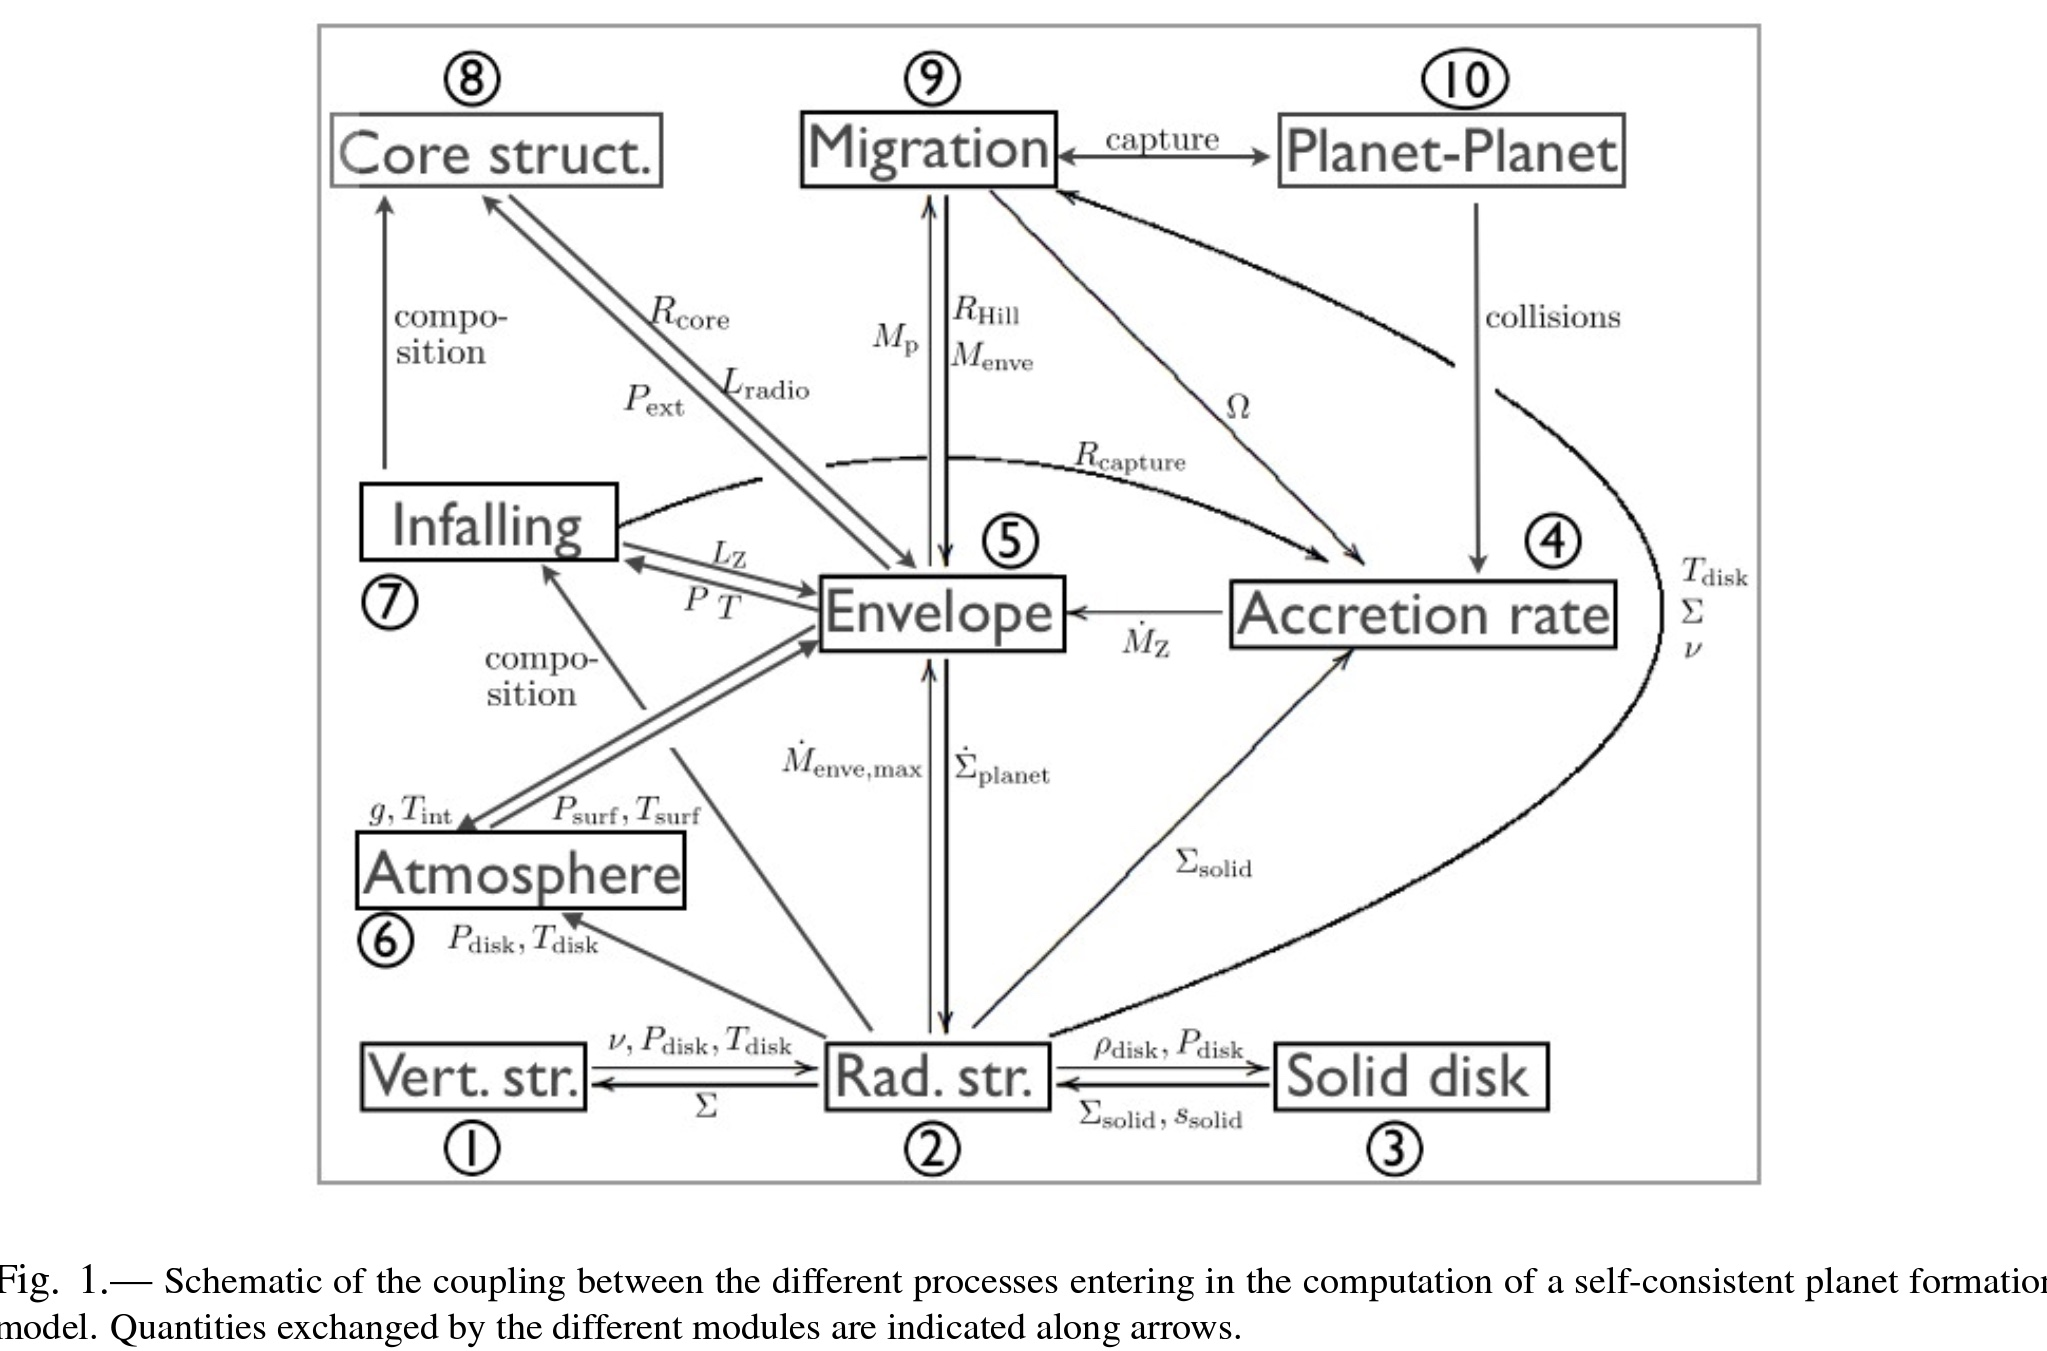
\includegraphics[trim={8cm 5cm 8cm 0},clip, keepaspectratio, width=0.7\textwidth]{GFM}
	\caption{Da \cite{benz2014planet}.}\label{fig:GFM}
\end{figure}
\end{frame}

\begin{wordonframe}{GFM}
contenu...
\end{wordonframe}

\begin{frame}{Distribuzione iniziale caratteristiche dischi protoplanetari}
	\begin{figure}[!ht]
		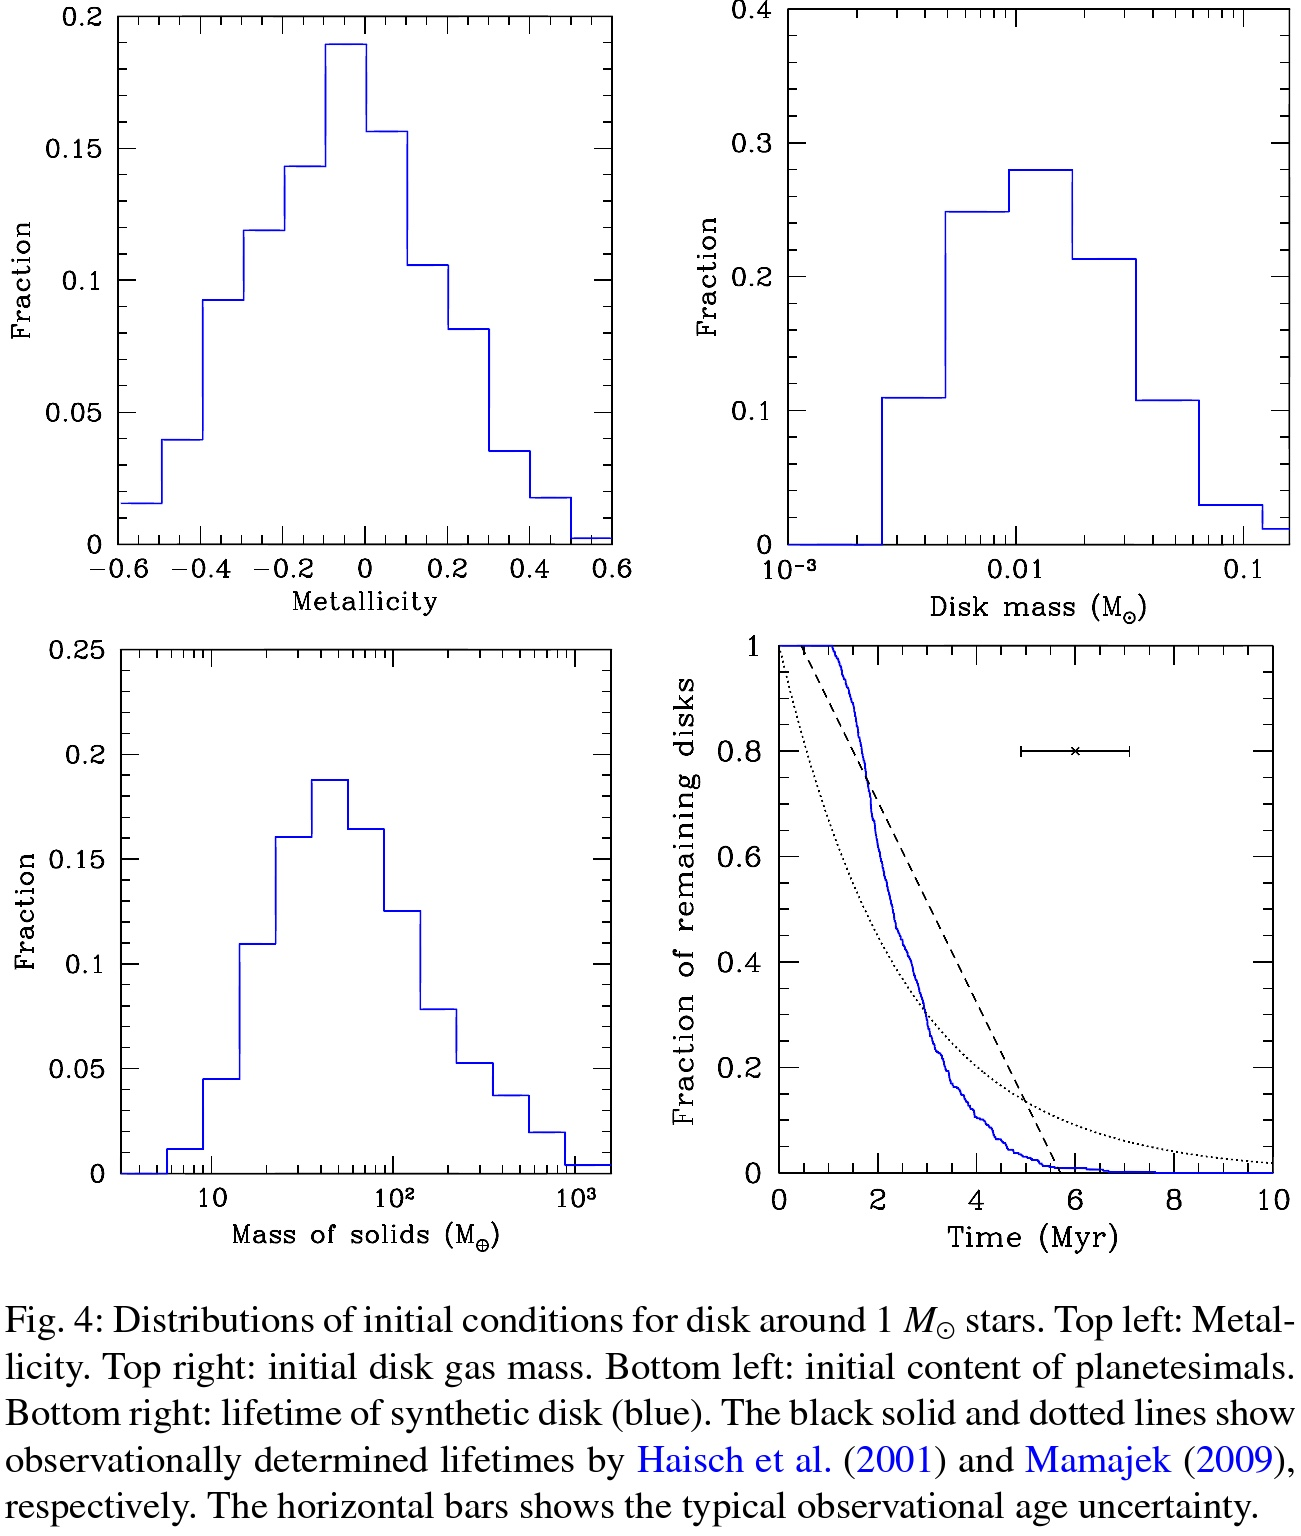
\includegraphics[trim={0cm 10cm 0 0},clip, keepaspectratio,width=0.7\textwidth]{initdistro}
		\caption{Da \cite{mordasini2018planetary}.}\label{fig:initdistro}
	\end{figure}
\end{frame}

\begin{frame}[allowframebreaks]{Condizioni iniziali ed evoluzione del disco protoplanetario}
\begin{block}{Evoluzione disco proto-planetario}
\begin{align*}
&\TDy{t}{\Sigma}=\frac{1}{r}\PDof{r}[3r\expy{1/2}\PDof{r}(\nu\Sigma r\expy{1/2})]+\dot{\Sigma}_w(r)+\dot{\Sigma}_{embryo}(r)\label{eq:diskaccrphev-m18}\\
&\dot{\Sigma}_w(a)=\left\{\begin{array}{c}0\\\frac{\dot{M}_w}{2\pi(a_{max}-R_g)a}\\\end{array}\right.\\
&\Sigma(a,t=0)=\Sigma_0(\frac{r}{1AU})\expy{p_g}\Exp{[-(\frac{r}{R_o})\expy{2+p_g}]}(1-\sqrt{\frac{r}{R_i}})
\end{align*}
\end{block}

\begin{block}{Parametri di montecarlo}
\begin{itemize}
	\item $M_{disk}$: distribuzione gaussiana di $\log{M_{disk}}$ ($\mu_{obs}=0.042\msun{}$, $\sigma_{obs}$)
	\item $\alpha$, $\dot{M}_w$: $t_{disk}(\alpha,\Sigma_0,\dot{M}_w)=\SI{3}{\mega\year}$.
	
	($\dot{M}_w=\SIrange{5e-10}{3e-8}\msun{}/\si{\year}$, $\alpha=\num{7e-3}$)
\end{itemize}
\end{block}

\end{frame}

\begin{wordonframe}{Evoluzione disco protoplanetario e condizioni iniziali}
La distribuzione di massa e la frazione di dischi protoplanetari per ammassi stellari di et\'a diversa \'e mostrata in figura (\ref{fig:initdistro}). La massa \'e determinata misurando il flusso di emissione termica della polvere: la distribuzione di $\log{M_{disk}}$  \'e gaussiana e per il cluster Ophiuchus la distribuzione \'e fittata da gaussiana con $\mu=-1.38$ ($M_{disk}=0.042\msun{}$) e $\sigma=0.49$.

Il tempo caratteristico del disco \'e determinato dalla viscosit\'a $\alpha$: fissata $\alpha$ compatibile con tempo caratteristico osservato $\tau_{disk}^{obs}\approx\SI{3}{\mega\year}$ e assumendo la distribuzione uniforme nel logaritmo di $\dot{M}_w$, si calcola  $t_{disk}(\alpha,\Sigma_0,\dot{M}_w)$ determinando gli estremi dello fotoevaporazione per riprodurre tempi di vita osservati.

Valori tipici sono $\dot{M}_w=\SIrange{5e-10}{3e-8}\msun{}/\si{\year}$ per $\alpha=\num{7e-3}$.

Nelle popolazione planetaria considerata $\alpha$ \'e fissato sulla base delle osservazioni  ed \'e omogeneo e costante.

\end{wordonframe}

\begin{frame}{Distribuzione iniziale planetesimi ed embrioni planetari}
\begin{block}{Conversione polvere in planetesimi}

	\begin{equation*}
	\Sigma_p(t=0,r)=f_{dg}\eta_{ice}\Sigma_g(t=0,r)
	\end{equation*}
	
	\begin{equation*}
	\frac{f_{D/G}}{f_{D/G\odot}}=10\expy{[\cel{Fe}{}{}{}/\cel{H}{}{}{}]}
	\end{equation*}
	$f_{D/G\odot}\approx\numrange{0.01}{0.02}$ (\cite{lodders2003solar}).
\end{block}
\begin{block}{Posizione iniziale embrioni e tempo di comparsa}
Posizione iniziale: $P(a)\,da\propto d\,\log{a}\propto\const{}$.
Tempo comparsa: accumulo massa planetesimi

\end{block}
\end{frame}

\begin{wordonframe}{Distribuzione iniziale planetesimi/embrioni}
---Distribuzione iniziale planetesimi
Assumendo conversione completa di polvere in planetesimi, la densit\'a superficiale di planetesimi \'e
\begin{equation}
\Sigma_p(t=0,r)=f_{dg}\eta_{ice}\Sigma_g(t=0,r)
\end{equation}
con $f_{dg}$ rapporto gas/polvere (circa metallicit\'a) \'e una parametro casuale con distribuzione che riflette distribuzione di metallicit\'a stellari, $\eta_{ice}$ tiene conto della discontinuit\'a nella distribuzione superficiale di solidi all'iceline.

Sulla scorta della piccola differenza tra composizione solare e composizione meteoritica e assumendo inoltre che il ferro sia un buon indicatore della componente solida  si usa la formula
\begin{equation}
\frac{f_{D/G}}{f_{D/G\odot}}=10\expy{[\cel{Fe}{}{}{}/\cel{H}{}{}{}]}
\end{equation}
con $f_{D/G\odot}\approx\numrange{0.01}{0.02}$ (\cite{lodders2003solar}).
\end{wordonframe}

\section{Caratteristiche popolazioni sintetiche}

\begin{frame}{Popolazione sintetica: traccie di formazione e fase accrescimento gas}

\begin{figure}[!ht]
	\begin{subfigure}[b]{0.48\textwidth}
		\centering
		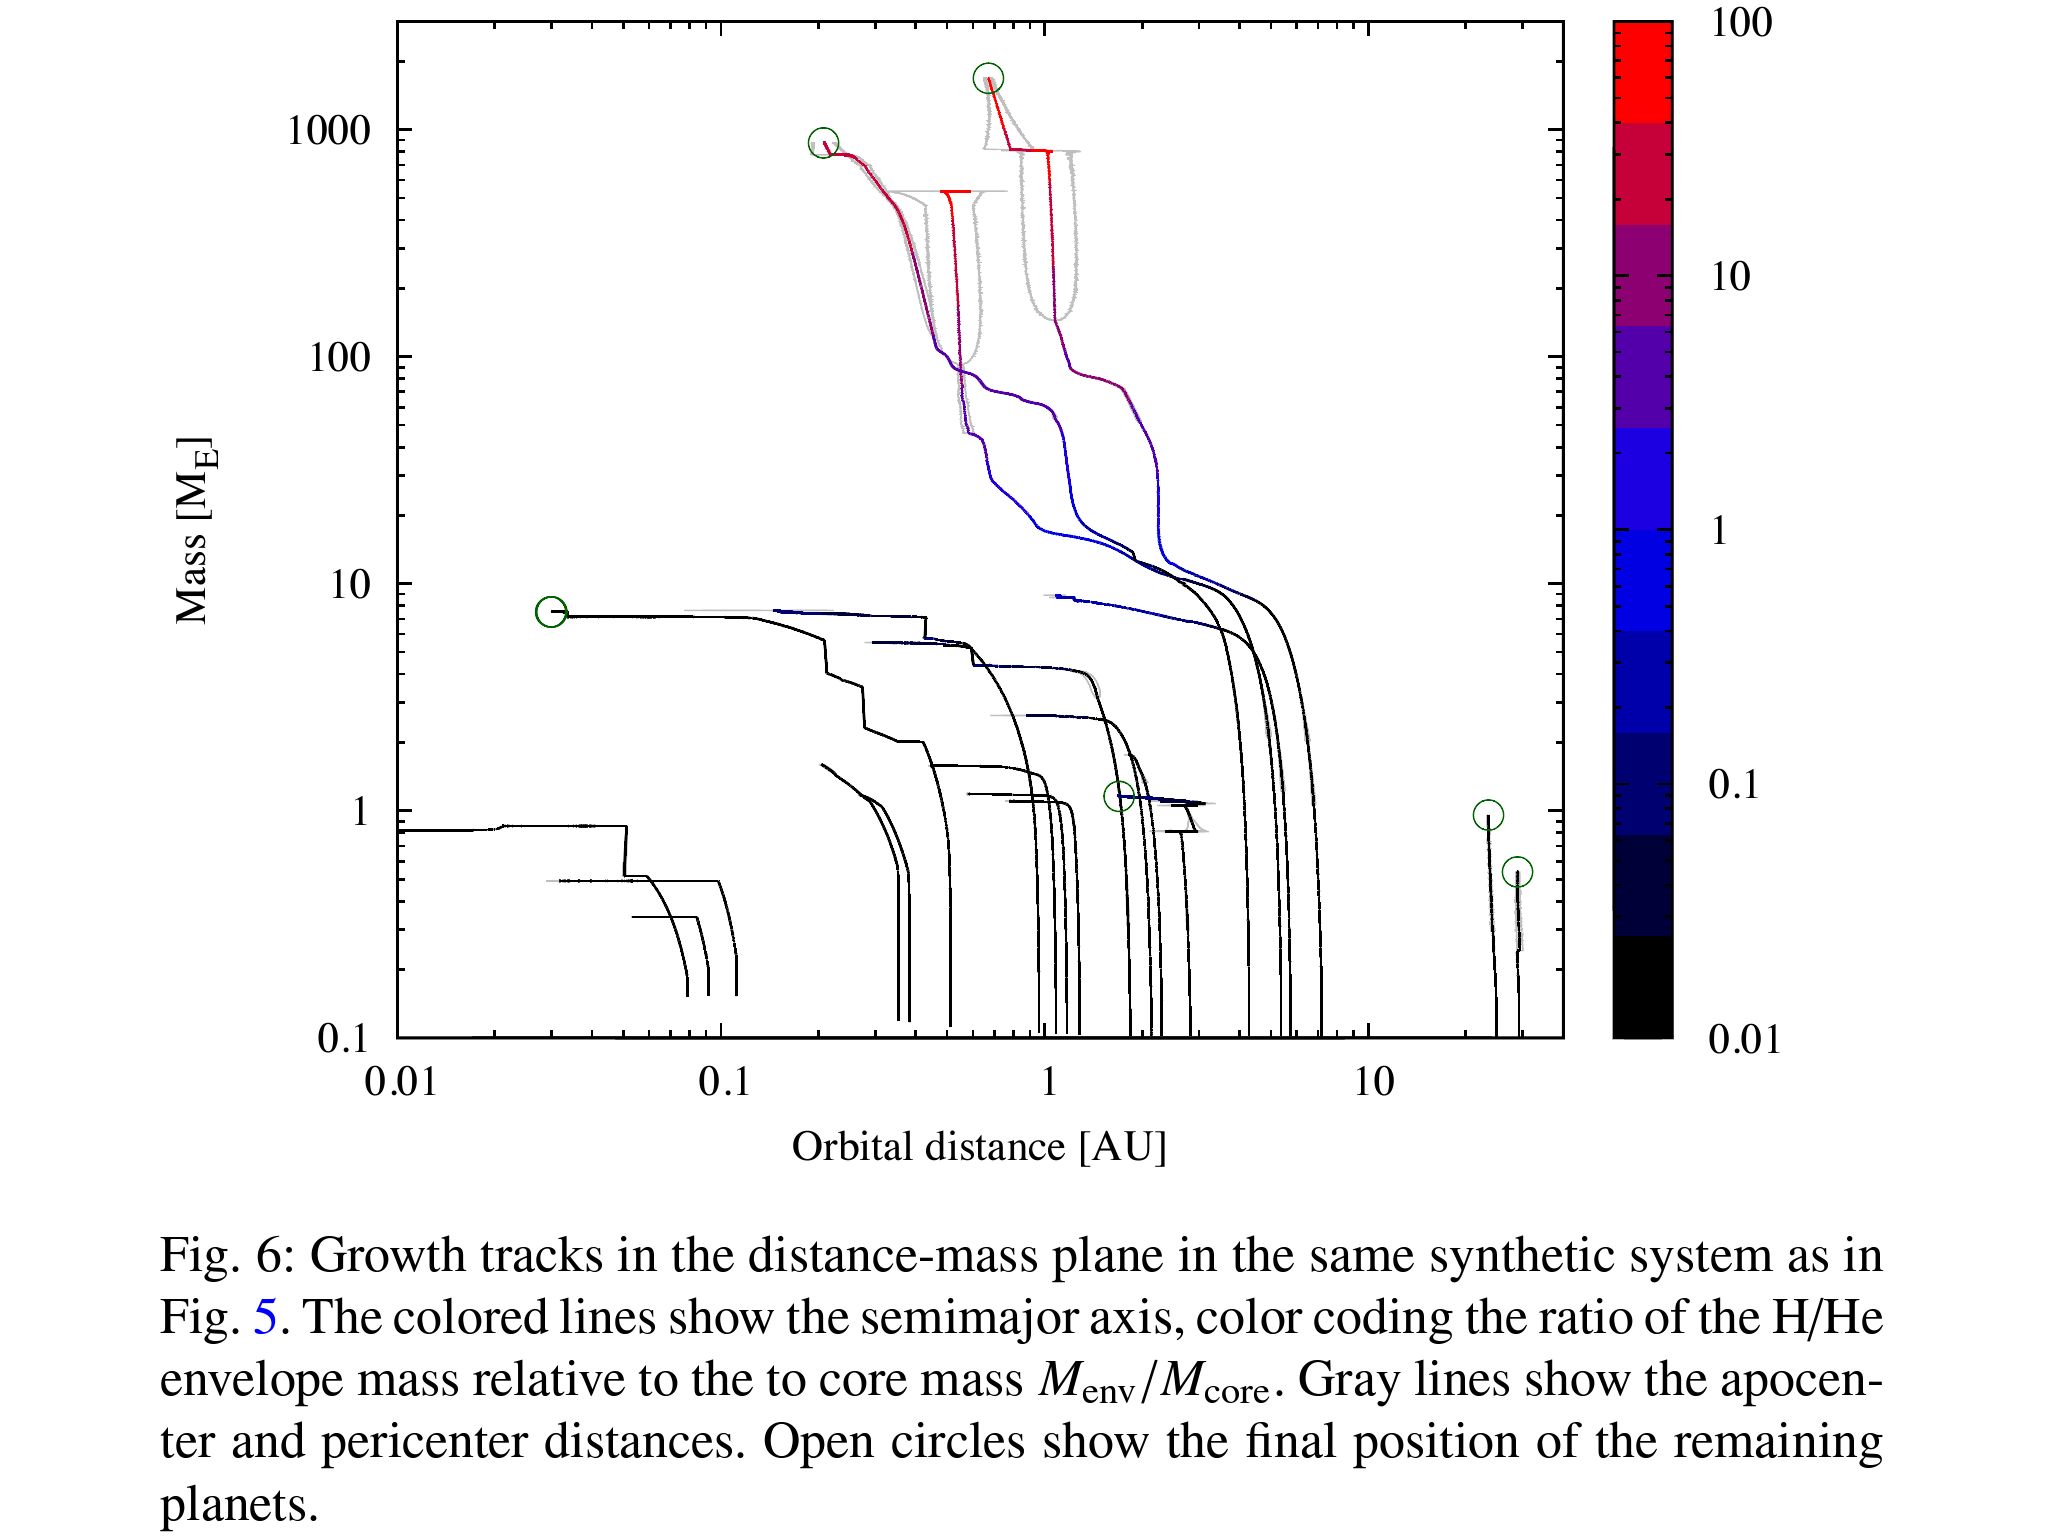
\includegraphics[trim={2cm 12cm 2cm 0},clip, width=0.99\textwidth,keepaspectratio]{track1}
		\caption{Formazione di un sistema planetario nel diagramma $a-M$: alla scomparsa del disco protoplanetario si hanno 2 pianeti giganti, un nettuniano caldo e 3 pianeti terrestri. La scala di colore indica la composizione $\frac{M_e}{M_c}$. Da \cite{mordasini2018planetary}.}\label{fig:track1}
	\end{subfigure}
	~
	\begin{subfigure}[b]{0.49\textwidth}
		\centering
		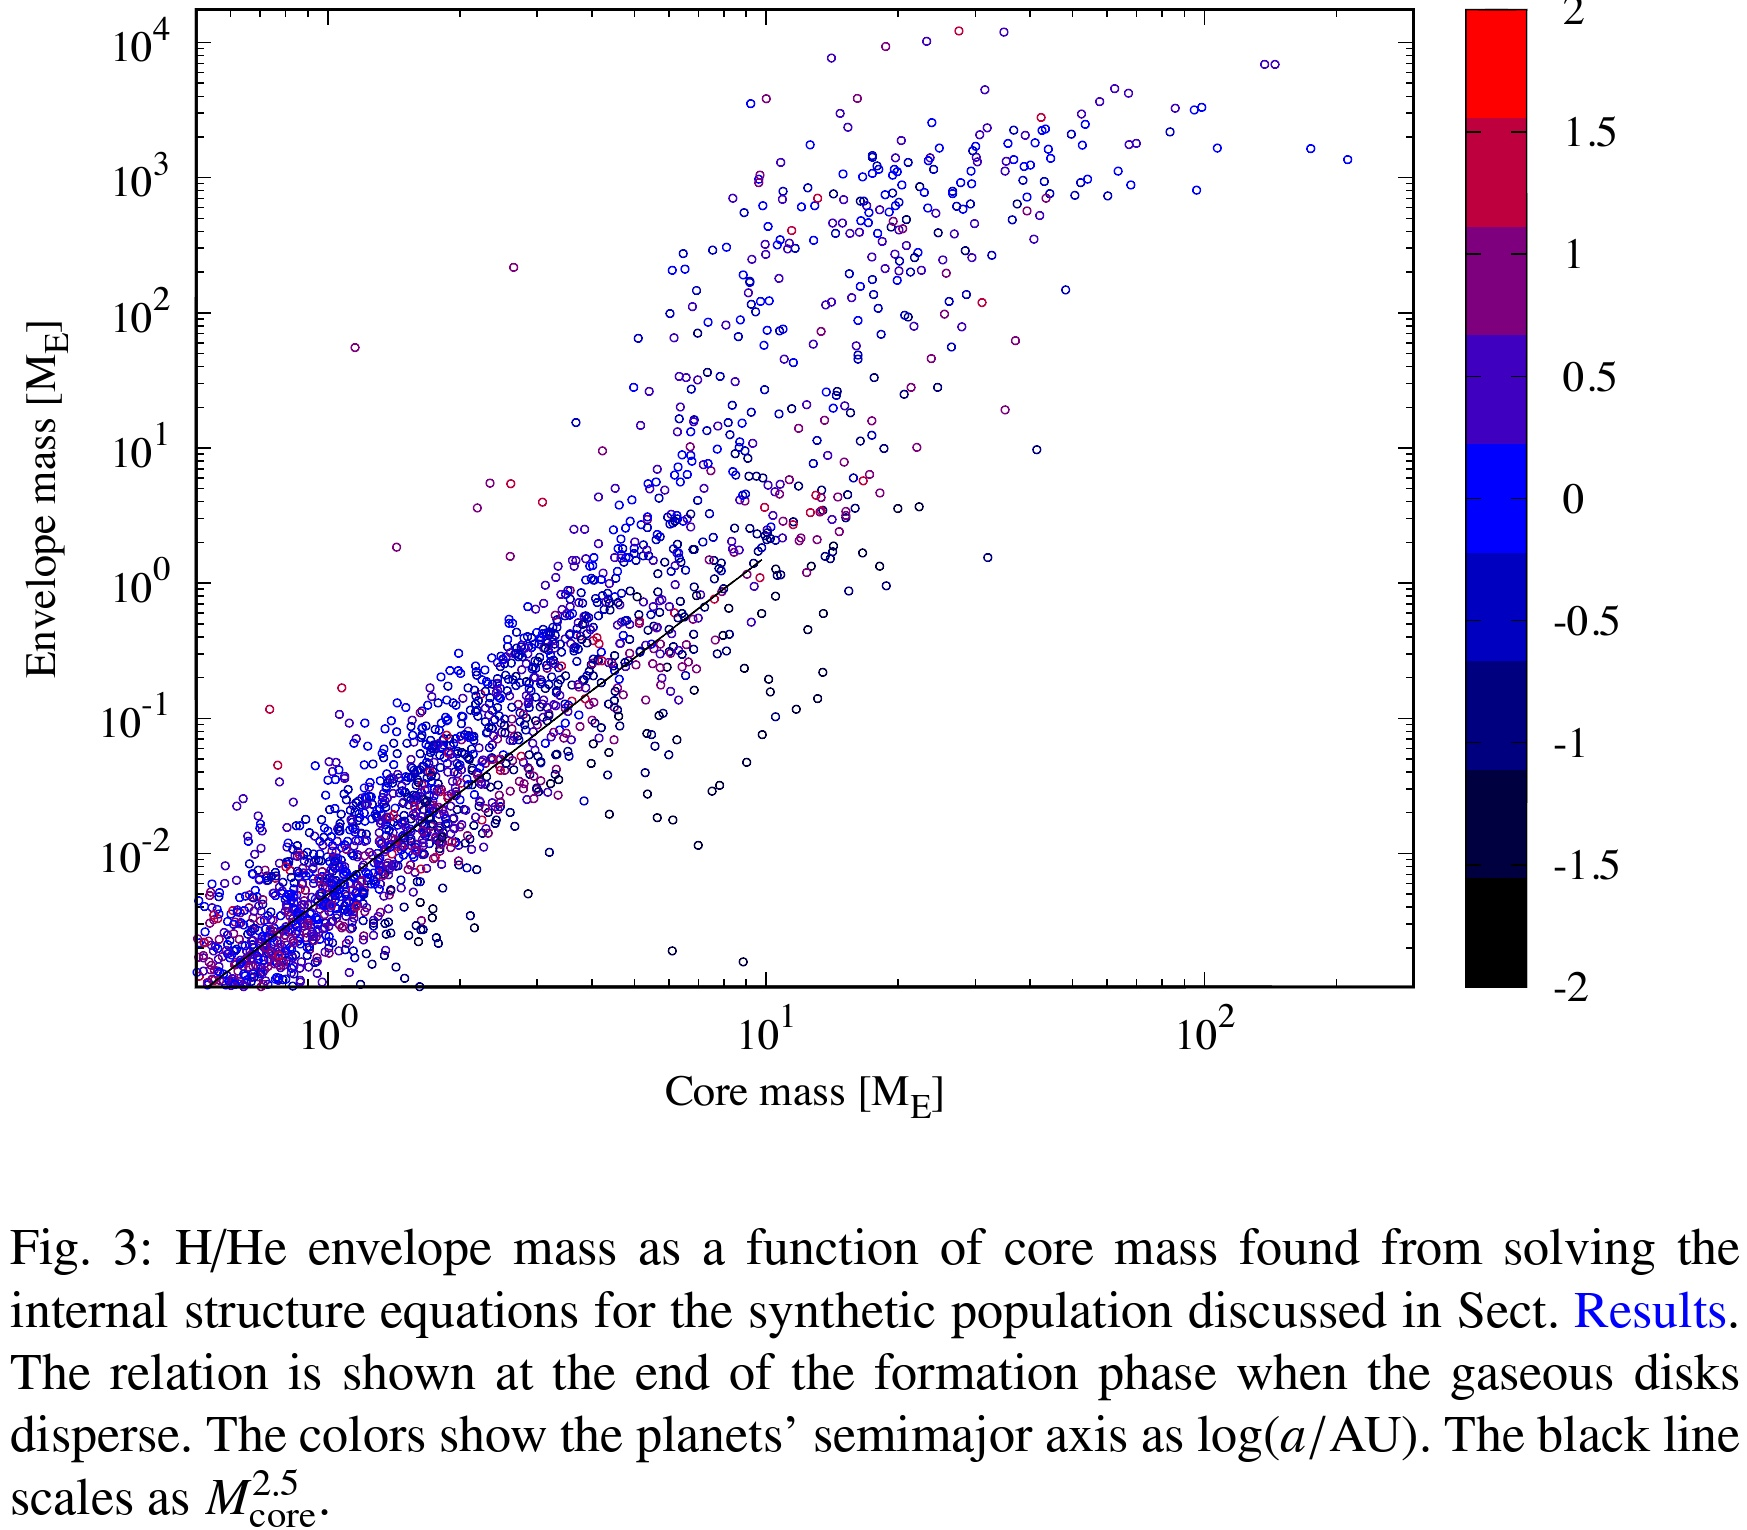
\includegraphics[trim={0cm 12cm 0 0},clip, width=0.99\textwidth,keepaspectratio]{envelopecoresynth}
		\caption{Massa inviluppo gassoso vs massa core. Il colore indica la distanza in $\log{\frac{a}{\si{\astronomicalunit}}}$. La linea continua mostra andamento $M_c\expy{-q_{KH}-1}=M_c\expy{2.5}$ precedente alla fase runaway di accrescimento gassoso. Da \cite{mordasini2018planetary}. }\label{fig:envelopecoresynth}
	\end{subfigure}
\end{figure}
\end{frame}

\begin{wordonframe}{Tracce formazione}
crescendo verso diversity in massa-distanza
\end{wordonframe}

\begin{frame}{Popolazione sintetica nel diagramma massa-distanza}
\begin{figure}[!ht]
	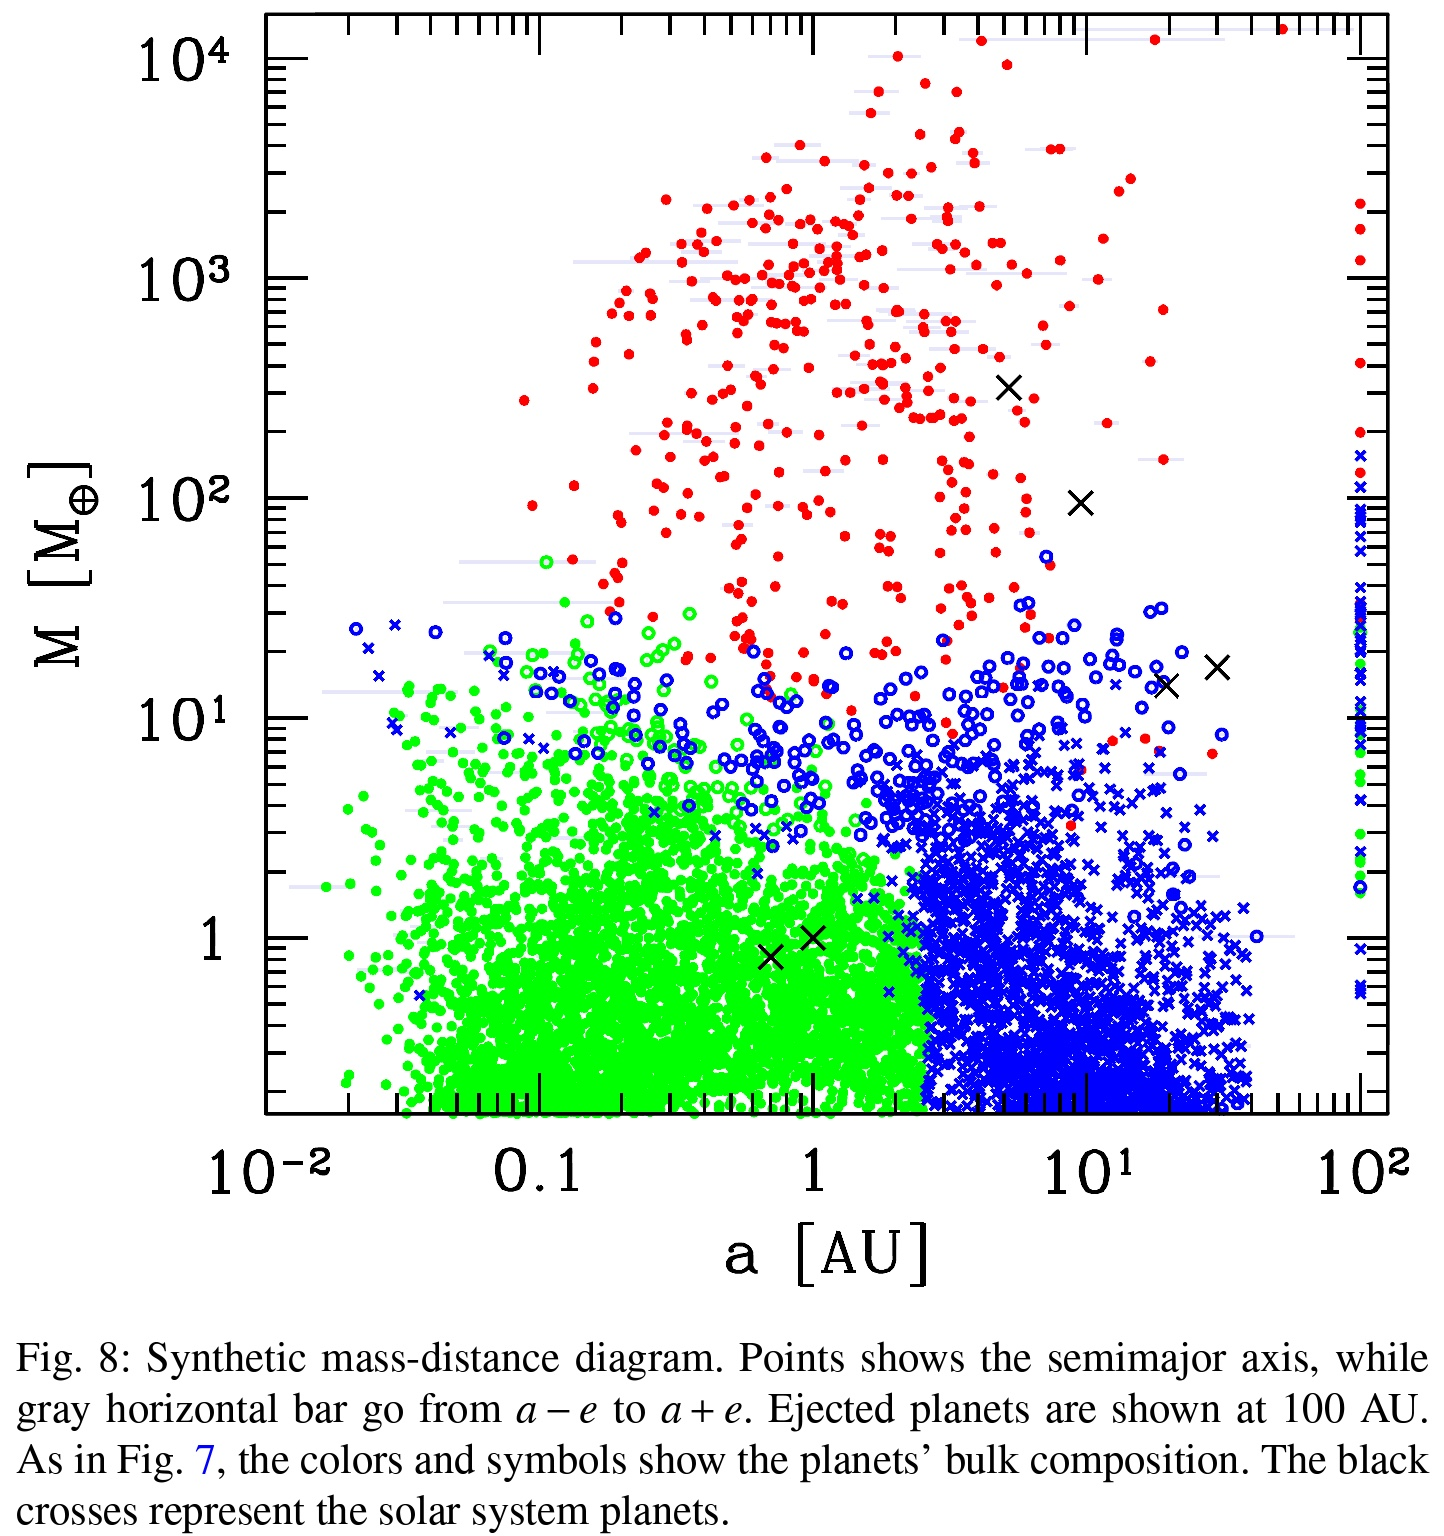
\includegraphics[trim={0cm 8cm 0 0},clip, width=0.8\textwidth,keepaspectratio]{ma-synth}
	\caption{Simulazione popolazione planetaria di 504 sistemi Punti rossi: pianeti giganti con $M_e/M_c>1$; simboli blu/verdi: pianeti che hanno accresciuto core con ghiacci/rocce; punti aperti: $0.1\leq M_{env}/M_{core}\leq1$; croci blu e punti pieni verdi: pianeti con $M_{env}/M_{core}\leq0.1$. Da \cite{mordasini2018planetary}.}\label{fig:ma-synth}
\end{figure}
\end{frame}

\begin{wordonframe}{diagramma M-a}

\end{wordonframe}

\section{Confronto semi-quantitativo simulazione-osservazioni}

\begin{frame}{Confronto pianeti giganti e sistemi compatti}
\begin{table}
	\begin{tabular}{|ccc|}
		\hline
		N&Giganti ($M>300\mearth{}$)&vicini ($P\leq100\si{\day}, R\geq\rearth{}$)\\
		\hline
		1&4.8&8.4\\
		2&7.4&12.8\\
		3&5.4&11.4\\
		4&0.4&10.0\\
		$\geq5$&0.0&11.4\\
		$\exv{S}$&18.0&54.0\\
		O&10-20&50-60\\
		\hline
	\end{tabular}
	\caption{Percentuale di stelle con N pianeti del dato tipo nella popolazione sintetica di \cite{mordasini2018planetary} e confronto con osservazioni.}\label{tab:planetfreq}
\end{table}

\begin{figure}[!ht]
	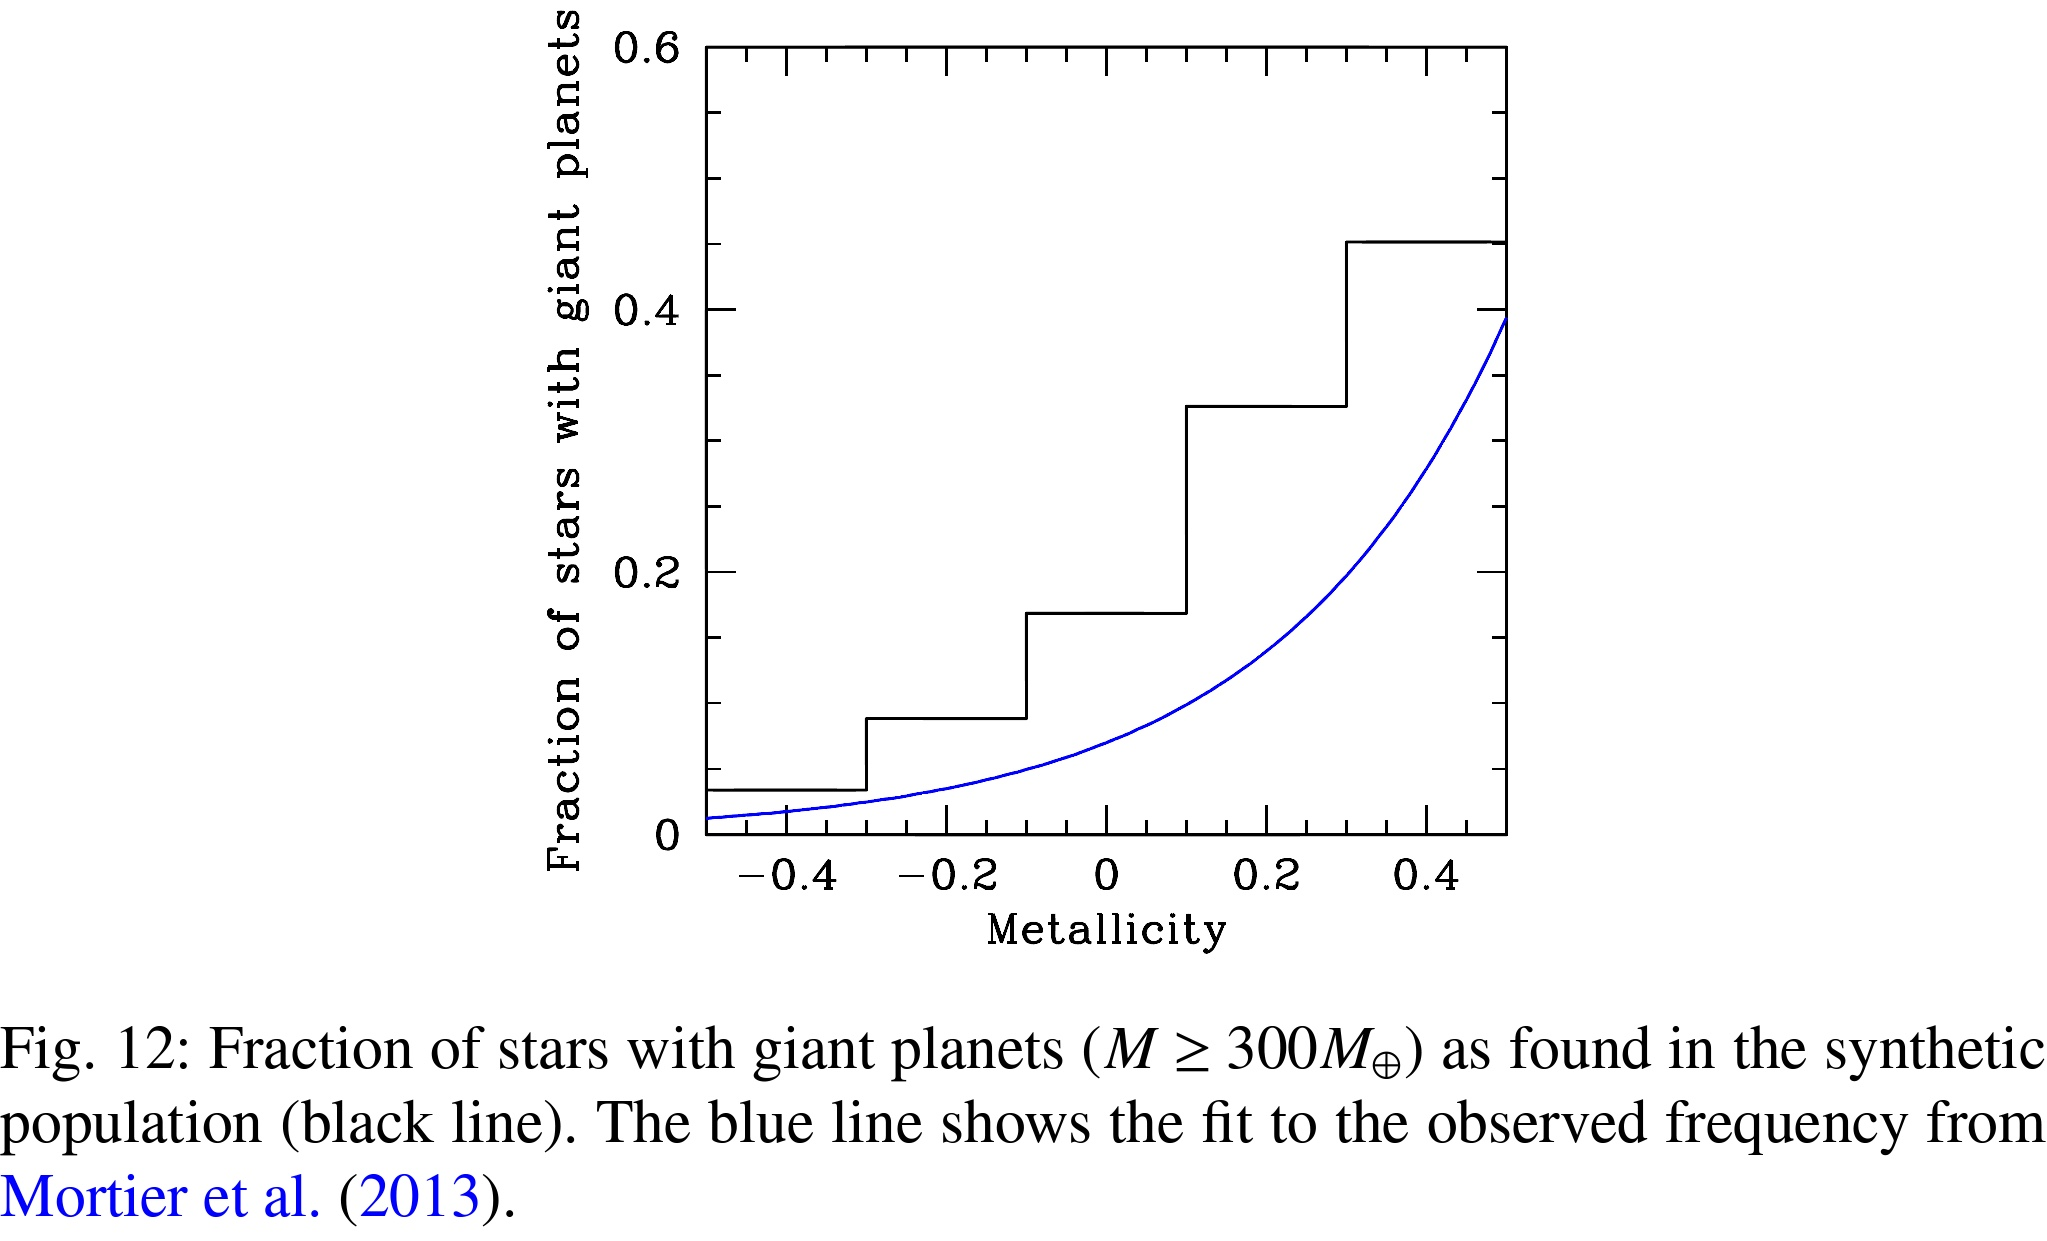
\includegraphics[trim={0cm 10cm 0 0},clip, width=0.9\textwidth,keepaspectratio]{giant-Zsynth}
	\caption{Distribuzione di stelle che ospitano pianeti giganti ($M\geq300\mearth{}$) in funzione della metallicit\'a. Nero: popolazione sintetica. Blu: fit da osservazioni. Da \cite{mordasini2018planetary}. }\label{fig:giant-Zsynth}
\end{figure}
\end{frame}

\begin{wordonframe}{Confronto giganti e compatti -Frequenza vs metallicit\'a}

\end{wordonframe}

\begin{frame}{Confronto pianeti giganti e sistemi compatti}
\begin{figure}[!ht]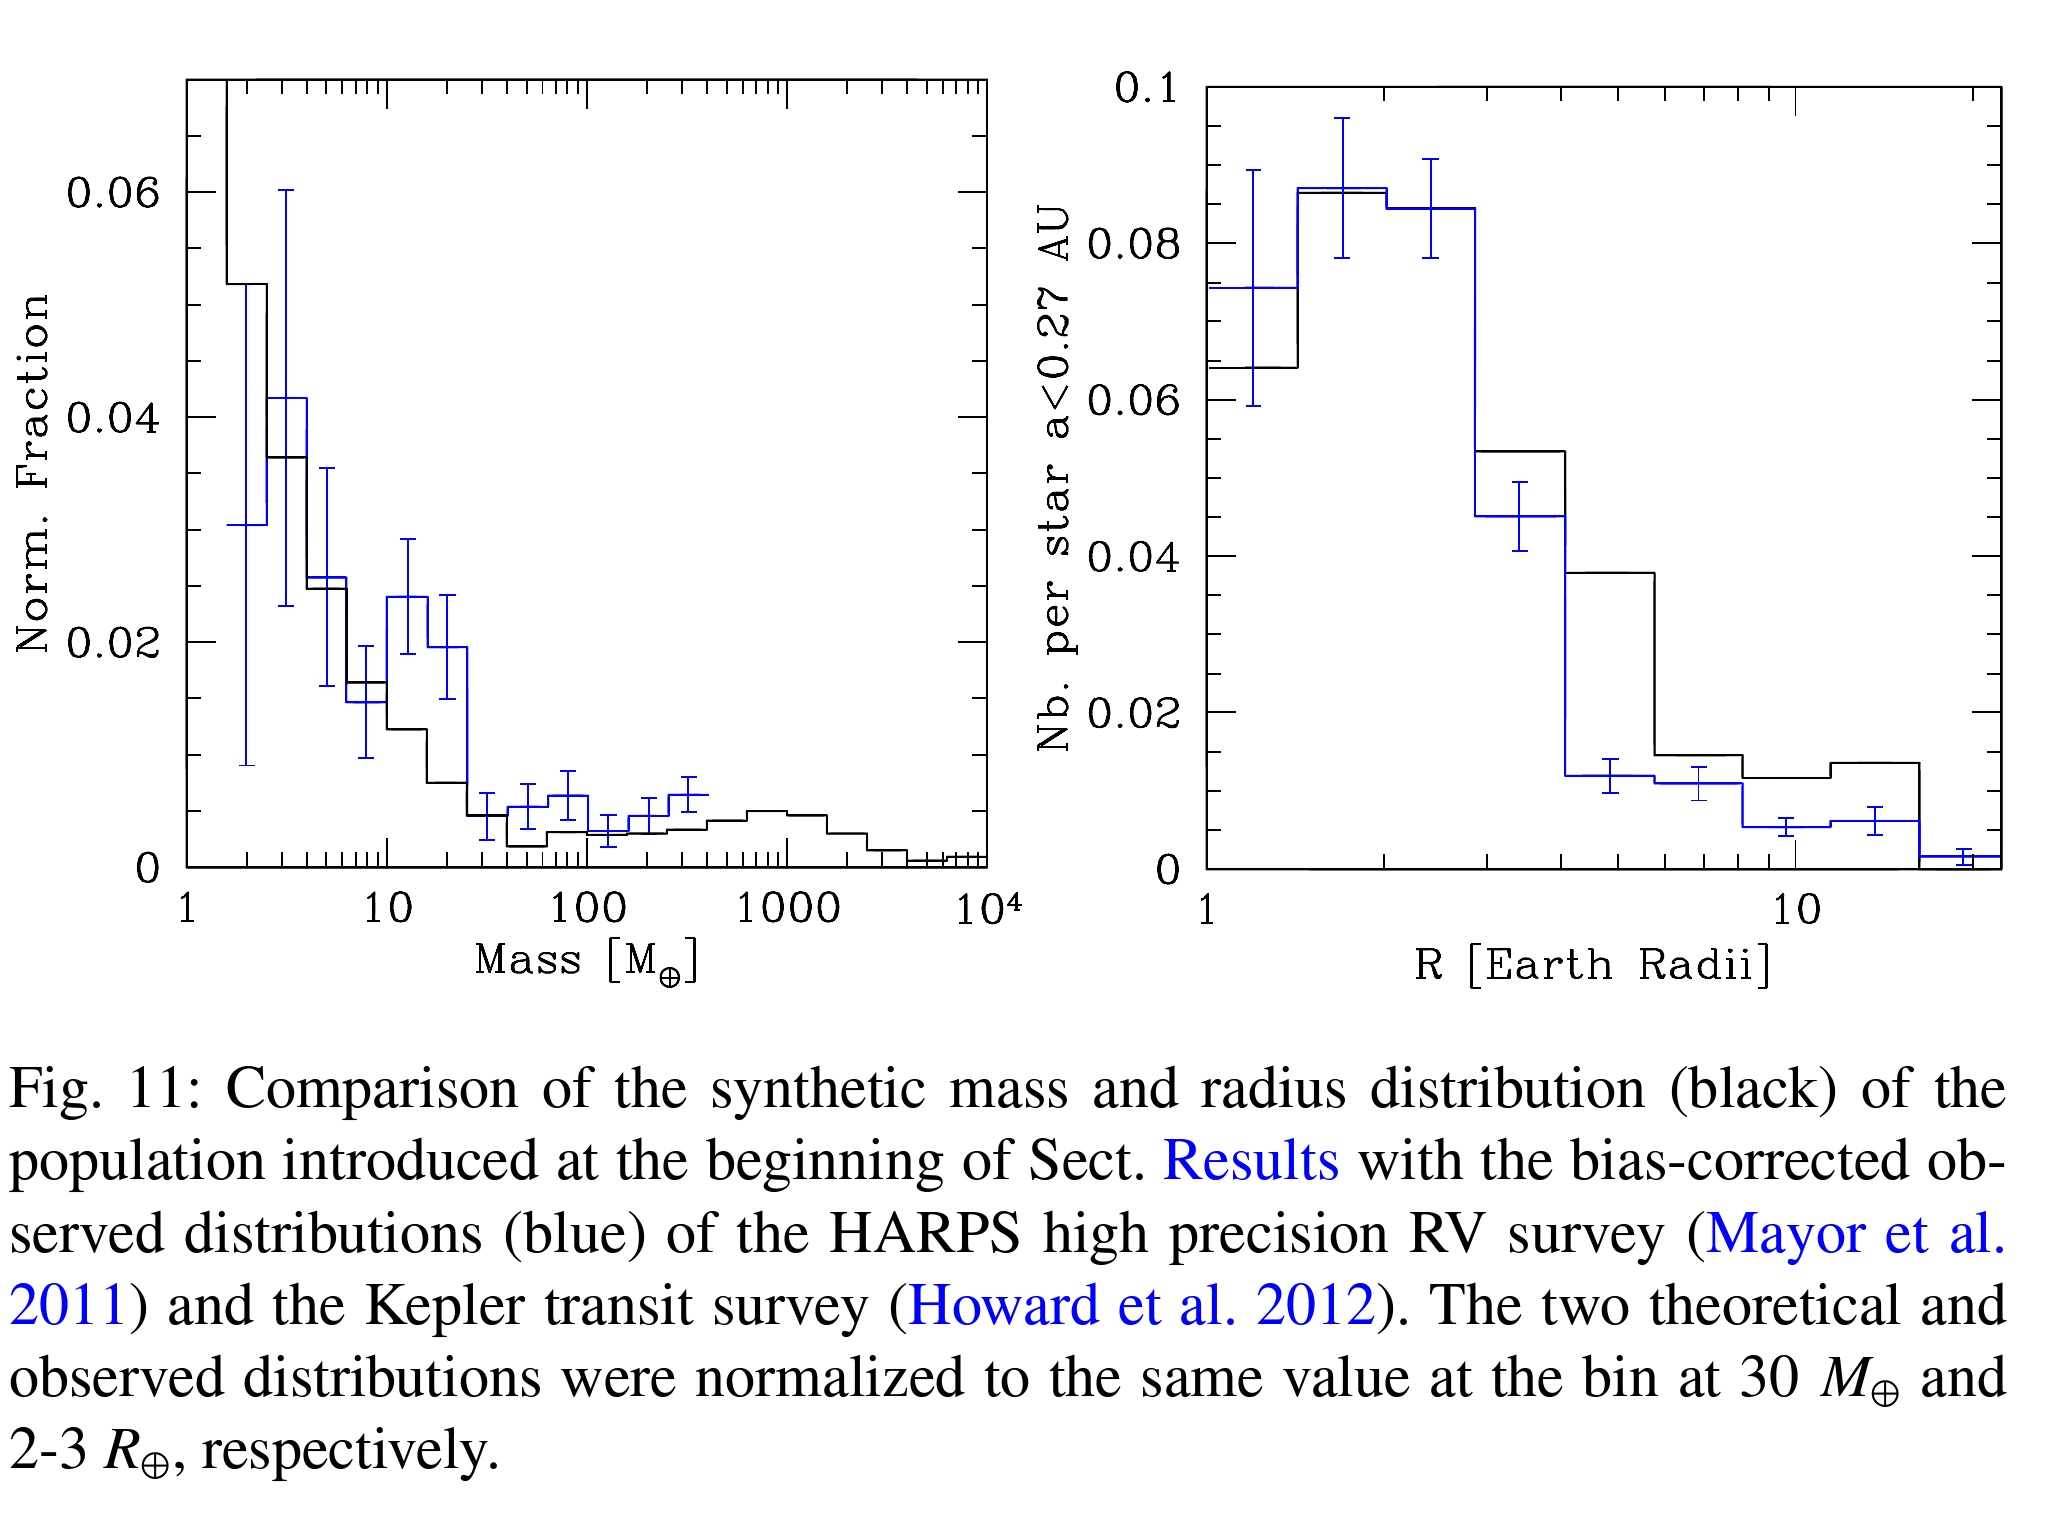
\includegraphics[trim={0cm 17cm 0 0},clip, keepaspectratio,width=0.9\textwidth]{MR-freq-obssynth}\caption{Distribuzioni di massa e raggio per popolazione planetaria sintetica (linea nera) e distribuzioni osservate tramite RV e transiti (linea blu) corrette per i bias. Da \cite{mordasini2018planetary}.}\label{fig:MR-freq-obssynth}\end{figure}
\end{frame}

\begin{wordonframe}{Confronto giganti e compatti -Frequenza vs metallicit\'a}

\end{wordonframe}


\end{document}